\documentclass[czech,bachelor]{../../shared/diploma}

\usepackage[autostyle=true,czech=quotes]{csquotes} % korektni sazba uvozovek, podpora pro balik biblatex
\usepackage[backend=biber, style=iso-numeric, alldates=iso]{biblatex} % bibliografie
\usepackage{dcolumn} % sloupce tabulky s ciselnymi hodnotami
\usepackage{subfig} % makra pro "pod-obrázky" a "pod-tabulky"
\usepackage{float} % lepsi umistovani obrazku (H)
\usepackage{xparse} % lepsi commandy s optional params
\usepackage{hyperref} % vkladani hypertextovych odkazu
\usepackage{enumitem} % lepsi enumerate a descrition and so on
\usepackage{wrapfig} % obrazky obtekané textem
\usepackage{latexsym} % symboly
% minted things
\immediate\write18{echo $ROAD > .ROAD.tex}
\immediate\write18{echo $ROAD "tohle je ten nejhorší hack co jsem kdy udělal"} 
\input{.ROAD}
\usepackage[outputdir=\ROAD]{minted} %
%\usepackage{minted}
\setminted{fontsize=\small, baselinestretch=1, frame=lines, framesep=8pt, linenos}
\renewcommand\listingscaption{Výpis}
\renewcommand\listoflistingscaption{Seznam výpisů zdrojového kódu}

\setcounter{tocdepth}{1}

% dark theme enable
%\usepackage{xcolor} \pagecolor[rgb]{0,0,0} \color[rgb]{1,1,1}

% Zadame pozadovane vstupy pro generovani titulnich stran.
\ThesisAuthor{Martin Korotwitschka}
\ThesisSupervisor{Ing. Radoslav Fasuga, Ph.D.}
\CzechThesisTitle{Tvorba API výpravné evoluční hry}
\EnglishThesisTitle{API Design for the Narrative Evolution Game}
\SubmissionYear{2024}
\ThesisAssignmentFileName{../specification.pdf}

% Pokud nechceme nikomu dekovat makro zapoznámkujeme.
\Acknowledgement{V první řadě bych chtěl poděkvoat všem členům týmu za aktivní spolupráci a zkušenosti získané na tomto projektu. Také bych chtěl poděkovat vedoucímu práce Ing. Radoslavu Fasugovi, Ph.D. za jeho vedení a rady. Dále svojí rodině a přátelům, bez kterých by bylo mé studium obtížné.}
\CzechAbstract{Tato práce se zabývá tvorbou aplikačního rozhranní pro hybridní výpravnou hru, které bude poskytovat koncové body pro administrativní rozhranní a pro rozhranní uživatele. Tato práce se nejprve zabývá analýzou možných způsobů řešení a implementace aplikačního rozhranní. Jako finální produkt by mělo vzniknout aplikační rozhranní které bude poskytovat koncové body ostatním spoluřešitelům. Společně s tímto aplikačním rozhranním by měla vzniknout i příručka popisující koncové body.}
\CzechKeywords{API; REST; RESTful; SOAP; GraphQL; JSON; HTTP; Databáze; výpravná hra; vývoj hry; Java; Spring Boot; }
\EnglishAbstract{This thesis deals with the creation of an application interface for a hybrid narrative game that will provide endpoints for the administrative interface and for the user interface. This thesis first discusses the analysis of possible ways of designing and implementing the application interface. The final product should be an application interface that will provide endpoints to other co-researchers. Together with this application interface, a manual describing the endpoints should be produced.

Translated with DeepL.com (free version)}
\EnglishKeywords{API; REST; RESTful; SOAP; GraphQL; JSON; HTTP; Database; adventure game; game development; Java; Spring Boot;}

%bib resource
\addbibresource{resources/sauce.bib}
\addbibresource{resources/impl.bib}


% Commandy pro snadnější psaní
\NewDocumentCommand{\chapterref}{mO{}}{(\hyperref[#1]{Kapitola \ref*{#1}#2})}
\NewDocumentCommand{\sectionref}{mO{}}{(\hyperref[#1]{Sekce \ref*{#1}#2})}
\NewDocumentCommand{\subsectionref}{mO{}}{(\hyperref[#1]{Podsekce \ref*{#1}#2})}
\NewDocumentCommand{\tableref}{mO{}}{(\hyperref[#1]{Tabulka \ref*{#1}#2})}
\NewDocumentCommand{\coderef}{mO{}}{(\hyperref[#1]{Výpis \ref*{#1}#2})}
\NewDocumentCommand{\figureref}{mO{}}{(\hyperref[#1]{Obrázek \ref*{#1}#2})}
\NewDocumentCommand{\listingref}{mO{}}{(\hyperref[#1]{Výpis \ref*{#1}#2})}


% Glossary stuff
\usepackage{glossaries}

\makenoidxglossaries
\loadglsentries{resources/glossary/glosset}

% Zacatek dokumentu
\begin{document}
\pagenumbering{roman}
% Nechame vysazet titulni strany.
\MakeTitlePages
\listoflistings
\clearpage
\listoffigures
\clearpage
\listoftables
\clearpage

% A nasleduje text zaverecne prace.
\pagenumbering{arabic}

\section{Úvod}\label{sec:api-goal}

Je důležité si uvědomit, že kvalitní návrh a pečlivá definice klíčových mechanismů projektu jsou základem pro úspěch jakéhokoli API. Tyto počáteční kroky určují strukturu a funkčnost API, které slouží jako zprostředkovatel mezi uživateli a systémem. Při návrhu API je třeba pečlivě zvážit, jaké typy operací a datových interakcí bude potřeba podporovat, aby byly splněny specifické potřeby aplikace.

\section{Jak na návrh}\label{sec:api-how}

Na samém začátku je klíčové pečlivě navrhnout, jaké funkce bude naše API nabízet a jak celkově bude aplikace fungovat. Musíme přesně specifikovat, jakou funkcionalitu od API očekáváme, protože na základě těchto požadavků definujeme koncové body. Tyto základní funkční požadavky následně použijeme jako výchozí bod pro návrh API a všech věcí okolo.

Tento obecný přístup k návrhu API bude nyní demonstrováno na příkladu naší hry, kde ukážeme praktické aplikace teoretických principů. Následovat bude detailní pohled na návrh a funkční požadavky specifické pro naši hru.


\section{Návrh API pro hru}\label{sec:api-design}

Jako první se může provést tzv. analýza funkčních požadavků.
\chapter{Historie a vývoj API}
\cite{apiHistory} Myšlenka API se již objevila už ve čtyřicátých letech minulého století, kdy Maurice Wilkes a David Wheeler vytvořili modulární softwarovou knihovnu pro EDSAC\cite{enwiki:1215865067} počítač
a s tím spojený dokument, který bychom v dnešní době nazvali jako API dokumentaci\cite{Wilkes1951}.
I když se tato dokumentace liší v mnoha ohledech od dnešních API dokumentací, tak je považována za jakýsi prototyp API dokumentací.

Poprvé se termín API v technické literatuře vyskytl v roce 1968 v článku \textit{datové struktury a techniky pro vzdálenou počítačovou grafiku}.\cite{art:fall_joint_computer_conference}
Pár let poté se tento termín vyskytl v oblasti databází.\cite{art:comparasion_of_the_application_programming_interfaces}
Výsledkem je definice API z roku 1990 vytvořená Carlem Malamudem: \textit{API = soubor služeb, které má programátor k dispozici pro provádění určitých úkolů.}\footnote[1]{Původní anglická definice zní takto: \textit{API = a set of services available to a programmer for performing certain tasks} }

Další fáze vývoje jakožto API založeného na webu byla disertační práce pana Roy Fieldinga\cite{phd:api_web_services}
, kde definoval REST jakožto tzv \textit{go-to protokol}, který umožňuje standardizovanou komunikaci mezi zařízeními na internetu.
Fielding představil nové pojetí api jakožto Web Programming interface, kdežto tradiční pojetí bylo API založené na knihovně. Tato disertační práce je základ pro dnešní pojetí webových API.

\endinput
\chapter{Formáty využívající se v API}
V této kapitole budou popsány především dva základní formáty dat které jsou stále aktivní -- JSON a XML.


\section{Serializace a deserializace} %TODO cote https://www.baeldung.com/cs/serialization-deserialization
Serializace a deserializace jsou důležité koncepty v programování. Umožňují ukládat, přenášet a znovu sestavit data. Používají se celou řadu věcí, jako je ukládání objektů do databáze, posílání dat po síti a nebo pro účely mezipaměťi.

Objekt má 3 základní vlastnosti: identitu, stav a chování. Stav reprezentuje jednotlivá data objektu.
\textbf{Serializace} je proces převádění stavu objektů do proudu bytů co mohou být kdekoliv uloženy nebo poslány. Tento proud může být poté zase rekonstruován do původního objektu. Pro serializaci si však muíme vybrat formát dat. Jako třeba JSON nebo XML. Ovšem používá se i binární reprezentace dat. Tato reprezentace se často využívá pro výkonnostní potřeby, protože jsou typicky rychlejší na zápis a čtení. Jejich nevýhoda ale je, že nejsou člověkem čitelné.

\textbf{Deserializace} je opačný proces od serializace. Tedy převedení proudu bytů zpátky do objektu.

Jednou z nevýhod serializace a deserializace jsou vysoké nároky na výkon. Můžeto trvat nezanedbatelné množství času. Zvlášť u velkých objektů. Za zmínku stojí i fakt, že ne všechny objekty mohou být serializovány. Jako třeba sockety nebo file handlery.


\section{JSON}
JavaScript Object Notation neboli JSON je formát, který je odvozen z Javascriptu, nicméně mnoho dnešních jazyků už má serializaci do JSONu zabudovanou interně. Jedná se o textový formát zápisu objektů, který je dobře čitelný člověkem. Ukládá data do párů \textbf{key:value} kdy key je klíč a value hodnota, která je pod ním uložená, obvykle může jít o číslo, textový řetězec, pole nebo i další objekt. Znaky v JSONu musí být v kódování UTF-8, ale formát podporuje i speciální znaky pokud jsou escaped, jako příklad můžeme uvést znaky \verb |\uD83D\uDE10| nebo \textit{neutral-face}. JSON je využíván primárně k výměně dat mezi webovými aplikacemi a servery, ale dá se používat i pro jednoduché databáze. Má prostá ale zato striktní pravidla a tudíž je jednoduché zkontrolovat jeho správnost. Jeden z jeho nedostatků je, že nemá podporu komentářů oproti XML, které tuto podporu má. \textbf{ TODO odkaz někde na iso normu https://www.iso.org/standard/71616.html} %TODO bibtech na iso normu plus dát emoji 😐 třeba xetex ale to se pak celé rozbije


\subsection{Pravidla}
\textbf{Key} neboli klíč daného objektu je vždy string a reprezentuje název určitého atributu. \textbf{Value} představuje hodnotu, kterou tento atribut nabývá a může být datového typu text, číslo, logická hodnota, null, další objekt či pole. Jednotlivé atributy jsou vždy odděleny čárkou. Jako příklad je uveden JSON objekt z API modelové hry, který popisuje hráče, jeho vlastnosti a jeho rasu, reprezentovanou jako vnořený objekt.

\begin{listing}[H]
  \inputminted{json}{resources/code/standards/player.json}
  \caption{Příklad JSON objektu}
  \label{code:json_player}
\end{listing}

V tomto JSONu můžeme vidět všechno, s čím se u tohoto datového formátu můžeme setkat. Jako první atribut, tento objekt má \verb|"id":4|, kde id je klíč a 4 je číslo -- to značí, že tento objekt má svůj unikátní identifikátor 4.

Na 6 řádku můžeme vidět atribut \verb|"title":"Elf"|. Value je v tomto případě text, který poznáme podle zaobalení uvozovek. Tento řádek v kontextu celého objektu značí, že se jedná o rasu postavy, která má název \textit{Elf}.

Atribut, který tento text zaobaluje, je \texttt{"race"}. Jedná se o příklad objektu, v tomto případě rasy, která má své vlastnosti reprezentované právě tímto objektem.

V atributu \texttt{"effects"} se nachází pole objektů. V tomto případě to jsou objekty obsahující klíč s id rasy a jejím efektem, ke kterému je přidána také informace o tom, od jaké úrovně je tento efekt zpřístupněn. Podobně tak na řádku 26 je jako value klíče \texttt{inventory} pole textových řetězců znázorňující předměty, které hráč vlastní.

Dále si můžeme povšimnout atributu \texttt{clazz} na řádku 3, který má hodnotu \texttt{null}. To nám značí, že tento konkrétní klíč u objektu zatím nic neobsahuje. Může se stát že jen nebyl přiřazen a v budoucnu nějakou hodnotu dostane.

A nakonec zde máme na řádku 29 atribut \texttt{dead} s hodnotou \texttt{false}. Tato hodnota značí logickou hodnotu, která má datový typ boolean. V našem případě se jedná o vlastnost, která nám říká, zda je hráč mrtvý (\texttt{true}) či nikoli (\texttt{false}).


\section{XML}
Extensible Markup Language je jazyk primárně určený na serializaci a přenášení dat, který je podobně jako JSON čitelný i člověkem. Základní stavební blok je node, atributy jsou uloženy do párů kterým říkáme tagy. Za pomocí své deklarace podporuje určení kódování a různé verze. Díky XML Schema definition také podporuje celou řadu datových typů a oproti JSONu podporuje i komentáře. Standardy spravuje společnost W3C. \textbf{fest fajny odkaz na w3c specifikaci do bibtex} %TODO bibtech na w3c


\subsection{Pravidla}
Na začátku dokumentu je vždycky XML deklarace, která určuje, o jakou verzi se jedná a jaké mají znaky kódování.
Samotná data jsou zaznamenána pomocí párových tagů, dohromady nazývaným \textbf{element}, které se zapisují jako počáteční (\texttt{<character>}) a ukončovací (\texttt{</character>}) tag, kde \textit{character} značí název atributu, podobně jako \textbf{key} u JSONu. Hodnota atributu se píše buď mezi počáteční a ukončovací tag, nebo přímo do tagu samotného (\texttt{<character id=4>}). Tzv. \textit{procesory} analyzují XML dokumenty a posílají dále strukturovaná data aplikaci, která se využívá. Procesory můžou být jak validující tak nevalidující, přičemž validující musí nalezenou chybu nahlásit ale pořád mohou v parsování pokračovat.

\begin{listing}[H]
  \inputminted{xml}{resources/code/standards/player.xml}
  \caption{Příklad XML dokumentu i se schématem}
  \label{code:xml_player}
\end{listing}

\begin{figure}[H]
  \centering
  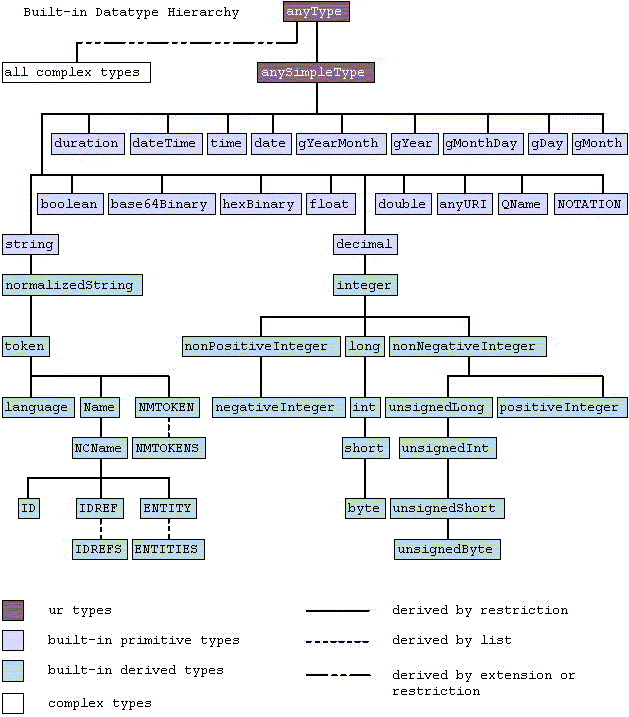
\includegraphics[width=0.7\textwidth]{figures/type-hierarchy.png}
  \caption{Hierarchie datových typů v XML schema}%\cite{british_museum_2021}}
  \label{fig:xml_datatypes}
\end{figure}
%TODO odkaz na obrázek všech možných datových typů https://www.w3.org/TR/xmlschema-2/type-hierarchy.gif a přímo ta stránka https://www.w3.org/TR/xmlschema-2/#built-in-datatypes


%TODO nějaký odkaz pěkný nebo tak něco na 
Tento XML dokument reprezentuje stejnou strukturu jako JSON popsaný výše. Oproti němu je však rozšířen o schéma, ve kterém můžeme určit jeden z mnoha datových typů \ref{fig:xml_datatypes} pro každý element (řádek 3) či atribut (řádek 6 a 7). Když není schéma specifikováno, všechny datové typy jou brány za text. Velká změna oproti JSONu také spočívá v tom, že víme, o jaký objekt se jedná (řádek 23 a 48) -- místo obyčejných složených závorek zde máme element se jménem \textit{character}, což je informace, kterou JSON neposkytuje.


\section{Shrnutí}
Teď byly představeny případné technologie co bychom mohli použít jako formát pro serializaci a deserializaci. Jak tyto technologie fungují, jak vypadají a jejich výhody a nevýhody.

\begin{table}[h]
  \centering
  \begin{tabular}{|l|c|c|c|c|}
    \hline
           & Čitelnost & Jednoduchost & Rychlost & Skladnost \\
    \hline
    JSON   & 1         & 1            & 2        & 3         \\
    \hline
    XML    & 2         & 3            & 4        & 4         \\
    \hline
    Binary & 5         & 4            & 1        & 1         \\
    \hline
  \end{tabular}
  \caption{Porovnání JSON, XML a Binary }
  \label{tab:formats_comparison}
\end{table}

\tableref{tab:formats_comparison} nám srovnává různé technologie podle našich případných požadavků. \footnote[1]{Známkování jsem prováděl čistě podle vlastního uvážení co bude pro naše použití nejvhodnější} \footnote[2]{Známkování je od 1 do 5 kdy 1 představuje souhlas a 5 nesouhlas} Pro naše účely je potřeba něco jednoduchého a srozumitelného, přiměřeně rychlého. Tedy nejlépe z toho vyplývá JSON. XML je pro naše účely moc komplexní a většinu vlastností nevyužijeme. Binární formát je sice rychlý ale špatně se odhalují chyby a je zde horší universálnost serializeru a deserializeru mezi jazyky.


\endinput
\chapter{Standardy využívané pro tvorbu API}\label{chap:standards}
V této kapitole si porovnáme a představíme různé architektury, které se používají pro tvorbu \gls{api}.
Hlavní často využívané nástroje, které si představíme, jsou \gls{rest}, GraphQL a SOAP.

\subsection*{Úvod}
\gls{api} je univerzální komunikační rozhraní mezi aplikacemi, které můžeme použít pro více druhů koncových aplikací. Ve své podstatě se jedná o soubor definicí, protokolů a občas i nepsaných pravidel.


\section{REST}\label{sec:rest}
\gls{rest}, což můžeme volně přeložit jako reprezentační stavový přenos, je nejčastěji používaná architektura API. Původně byl vytvořen jako vodítko, jak modelovat komunikaci po Internetu, jeho popularita však dále rostla z důvodu jednoduchosti implementace, flexibility z pohledu provádění změn, výkonnosti a přehlednosti i ve velkých projektech.

Webové služby, které pro své API využívají architekturu REST, jsou nazývány RESTful webové služby. Pojem \gls{restful api} většinou označují RESTful web API. Nicméně tyto dva pojmy se mohou zaměňovat nezávisle na sobě. \cite[]{devToApiStyles}


\subsection{Principy \gls{restful api}}\label{sec:rest:principles}

Níže jsou popsány základní principy, které \gls{restful api} dodržují.\cite{restfulApi}\cite[]{phd:restful_api}

\subsubsection*{Uniform interface}
Jedná se o klíčovou vlastnost RESTful služeb, která indikuje, že server předává a přijímá data v určitém specificky strukturovaném formátu. Nejčastěji se jedná o JSON nebo XML, ale může to být i jiný formát.

Jednotné rozhraní by mělo dodržovat následující pravidla.\
\begin{itemize}
    \item Požadavky by měly identifikovat zdroje.
    \item Klient je schopen z přijatých dat provést úpravu nebo smazání dat.
    \item Klient je schopen přijmout metadata o tom, o jaký typ zprávy jde a podle toho zjistit, jak tuto zprávu zpracovat.
    \item Klient může dostat informace o ostatních datech, která se vážou k původnímu požadavku. (\gls{hateoas})
\end{itemize}

\subsubsection*{Stateless}
Bezstavová komunikační metoda je taková metoda, kdy server obslouží každého klienta zvlášť a nezávisle na jeho předchozích akcích. Klienti mohou dávat požadavky nezávisle na pořadí, server si tedy neuchovává data o klientech.

\subsubsection*{Layered system}
U tohoto stylu architektury se klient může připojit i k jiným zprostředkovatelům a pořád dostane odpověď od serveru. Servery se taktéž mohou dotazovat na jiné servery při zpracovávání požadavků od klienta, tímto způsobem tedy můžeme mít systém rozdělen do více vrstev, jako je bezpečnostní vrstva, aplikační vrstva či business logika, přičemž tyto vrstvy zůstávají pro klienta skryté.

\subsubsection*{Cacheability}
Velká výhoda RESTful webových služeb je ta, že podporují cache. V tomto případě server označuje data jako cacheable či non-cacheable, přičemž při stejném dotazu klienta vícekrát za určitý čas se pro cachable data použijí již stáhnutá data. Dobrým příkladem využití je u obrázků, kde je server nemusí pokaždé načítat znovu a tím docílí rychlejší odezvy.

\subsubsection*{Code on demand}
Posledním ze standardů je možnost, že server může vrátit kód, který má klient vykonat, pomocí čehož může server rozšířit klienta o funkcionalitu, například při validaci formuláře se uživateli může ihned zobrazit chybová hláška. Dnes se však tento standard až tak často nevyužívá.


\subsection{Komunikace přes \gls{restful api}} % TODO reformat this bcs its not the same as rest
\gls{restful api} funguje na protokolu HTTP/S. Klient nejprve pošle serveru požadavek strukturovaný podle dokumentace konkrétní API. Server u požadavku zkontroluje, zda je klient oprávněn tuto operaci provést, a následně ho zpracuje odpovídajícím způsobem a klientovi vrátí odpověď s příslušným stavovým kódem.

\subsubsection*{Message body}
Ať už jde o požadavek či odpověď, pokud je třeba přenášet větší množství dat, většinou jsou vložena do message body. Jedná se o čistě textovou reprezentaci dat, jejíž formát není nikde specifikován a je na programátorech samotných, jaký si zvolí. Nicméně nejčastěji se používá výše zmíněný JSON nebo XML.

Například při požadavku GET pro uživatele s ID 1 server vrátí v message body JSON
\begin{verbatim}
	{"name": "Jožko Mrkvička", "age": 30}
\end{verbatim}
Tento objekt reprezentuje uživatele, který se jmenuje Jožko Mrkvička a je mu 30 let.

\subsubsection*{Headers}
V hlavičce požadavku a odpovědi se nachází dodatečné informace. Může se jednat o kódování body, datum a čas, typ obsahu v body, nebo autorizaci na straně klienta jako třeba session key.


\subsection{Požadavky}
Požadavky na \gls{restful api} musí obsahovat následující.

\subsubsection*{URI}
Unique resource identifier je unikátní identifikátor pro určitá data. V kontextu \gls{restful api} se nejčastěji jedná o URL, kterému se taktéž říká endpoint -- specifikace cesty k daným datům.

\subsubsection*{Metoda}
Jak již bylo zmíněno výše, \gls{restful api} typicky používá HTTP/S protokol, z něhož také přebírá metody pro komunikaci, které jsou zde ve zkratce rozepsány.

\begin{itemize}
    \item GET -- Požadavek pro získání dat na základě parametrů v URL. Opakované volání vrátí vždy stejný výsledek.
    \item POST -- Požadavek pro vložení kompletně nových dat, přenášených v message body. Opakované volání této metody vrátí pokaždé jiný výsledek.
    \item PUT -- Požadavek pro úpravu dat, opět vložených do message body. Opakované volání vrátí vždy stejný výsledek.
    \item DELETE -- Požadavek pro smazání dat.
    \item PATCH -- Požadavek pro částečnou úpravu dat. Není třeba posílat celý objekt, ale pouze změny.
\end{itemize}


\subsection{Odpovědi}
REST principy vyžadují, aby v odpovědi byly obsaženy následující prvky.

\subsubsection*{Stavové kódy}
Stavové kódy slouží k rychlé identifikaci toho, daný požadavek dopadl, zda-li bylo vyhodnocení úspěšné nebo se vyskytla chyba. Jejich struktura je pevně daná a její správné použití je základem dobře a efektivně vedené komunikace. Stav je trojmístné číslo, kde je podle počáteční číslice zaznamenán typ odpovědi a následující dvě cifry už slouží k identifikaci jednotlivých stavů v dané kategorii. Kód začínající 2xx značí úspěch, 4xx chybu na straně klienta, 5xx chybu na straně serveru a v neposlední řadě 3xx označuje přesměrování URL.

Nejčastěji využívané kódy jsou tyto:

\begin{itemize}
    \item 200 OK -- Vše proběhlo v pořádku.
    \item 201 Created -- Vše proběhlo v pořádku při požadavku POST (data byla zapsána).
    \item 400 Bad Request -- Server nepřijímá tato data, chyba je na straně uživatele.
    \item 401 Unauthorized -- Klient nemá potřebná oprávnění pro vykonání této akce.
    \item 404 Not Found -- Adresa či data, na které se klient dotazuje, neexistují.
    \item 500 Internal Server Error -- Obecná chyba na straně serveru.
\end{itemize}


\subsection{Shrnutí}
REST je dnes obecně nejpoužívanější architektura pro API. Je velice flexibilní, jednoduchá a programátor si může sám určit, který formát pro přenos dat bude používat. Je také velice intuitivní a samopopisný, takže není náročný na naučení. Nicméně kvůli textové podobě přenosu dat může být pomalejší než architektury používající binární soubory, což je však možné optimalizovat pomocí cache. \cite[]{devToApiStyles} \cite{phd:restful_api}\cite{restfulApi}


\section{SOAP}
SOAP neboli Simple Object Access Protocol je další z mnoha architektur API. Taktéž využívá primárně aplikační vrstvu HTTP/S, ale je možné ho použít i nad jinými protokoly. Je postaven na XML formátu.


\subsection{Charakteristika}
SOAP je založen na třech základních stavebních kamenech, které definují strukturu přenášených zpráv. \cite{soap}\cite{enwiki:1192016676}

\begin{itemize}
    \item Envelope -- Zapouzdřuje celou zprávu, určuje jakou strukturu má zpráva mít a jak ji zpracovat.
    \item Header -- Obsahuje informace o zprávě jako jsou například autentizační údaje.
    \item Body -- Samotná data, obsahují informace, které se mají přenést, ať už se jedná o dotaz nebo odpověď.
    \item (Fault message) -- Nepovinná část, která obsahuje kód chyby, aktéra, textový řetězec a detail.
\end{itemize}

Z pohledu klienta je SOAP velmi podobný RESTful architektuře. Klient vygeneruje požadavek ve formátu XML a ten pošle na SOAP server, čímž vyvolá požadovanou aplikaci běžící na něm. Odpověď serveru s požadovanými daty, parametry a hodnotami přepošle nejdříve SOAP request handleru, odkud je následně předána klientovi.

\subsection{Výhody}

SOAP je \textbf{nezávislý na platformě}. Neboli může běžet na jakémkoli operačním systému či síťovém protokolu, což umožňuje komunikaci mezi různými jazyky jak na Windows tak i Linuxu.

Primárně se používá \textbf{HTTP protokol}, což přináší výhodu, neboť zde není třeba upravovat firewall, ale funguje na jakémkoli protokolu, kde je však nutné komunikační infrastrukturu upravit.

Soap je velice \textbf{zabezpečený} -- má vlastní rozšíření Web Services Security, které podporuje bezpečnostní funkce jako x.509 certifikáty, vývojáři definované tokeny, Kerberos tickety a prověření uživatele pomocí ID a hesla. Jak již bylo zmíněno, i samotná podpora HTTP protokolu přidává vrstvu šifrování.

\subsection{Nevýhody}
\begin{itemize}
    \item Rychlost -- Kvůli vysokému zabudovanému zabezpečení a serializaci do XML je tento protokol velice pomalý v porovnání s ostatními.
    \item Složitost -- Vzhledem k podpoře více protokolů je nemožné plně využít funkcí jednotlivých protokolů jak je tomu u RESTful, například cachování nebo Uniform interface.
\end{itemize}


\subsection{Shrnutí}
Vzhledem k masivnosti a rychlosti tohoto protokolu se od něj upouští, aby se optimalizovala rychlost tvořených API. To však neznamená, že se už nepoužívá -- díky jeho bezpečnosti je stále využíván bankami, v E-komerci, zdravotnictví a všude, kde je primární apel na bezpečnost. \cite{soap}\cite{enwiki:1192016676}


\section{GraphQL}
GraphQL byl vyvinut Facebookem, dnes již známým pod názvem Meta. Jedná se o open-source dotazovací jazyk a prostředí pro běh programu určený pro API, který poskytuje deklarativní získávání dat, u kterého si klient přesně určí jaká data potřebuje. Je tedy velice šetrný k datům a snižuje nutnost mít více endpointů pro různě rozdělená či vyplněná data. Díky tomu, že GraphQL může načítat data z různých zdrojů, také není závislý na konkrétní databázi či úložišti.


\subsection{Design}
GraphQL je postaven na principu vrácení pouze těch dat, o které si klient řekne, bez nadměrného nebo nedostatečného načítání, což celkově zrychluje přenos dat. Pro definici prostředků využívá typový systém nazvaným schéma, proti kterému je zkontrolována query každého požadavku a až poté je vykonána. Server potom vrátí data ve stejném formátu jako zadaná query, typicky se používá JSON. Níže jsou popsány nejdůležitější stavební kameny GraphQL. \cite{enwiki:1219709983} \cite{graphqlOfficial}

\begin{listing}[ht!]
    \inputminted[]{ts}{resources/code/standards/playertype.gql}
    \caption{Příklad schématu v GraphQL}
    \label{code:gql_type}
\end{listing}

\begin{listing}[ht!]
    \inputminted[]{graphql}{resources/code//standards/playerquery.gql}
    \caption{Příklad query v GraphQL}
    \label{code:gql_querry}
\end{listing}


\begin{listing}[h]
    \inputminted[]{graphql}{resources/code/standards/types.example.gql}
    \caption{Příklady datových typů}
    \label{code:gql_datatypes}
\end{listing}

\begin{itemize}
    \item Type system \sectionref{sec:graphql:datatypes} -- Základ typového systému je Query, která určuje, jaké objekty mohou být získány \coderef{code:gql_type}[, řádek 29]. Vlastnosti ve výchozím stavu mohou nabývat hodnotu \texttt{null}. Za datový typ se může dát vykřičník abychom označili že tato hodnota nikdy nebude \texttt{null}.
    \item Queries \subsectionref{sec:graphql:query} -- Query přesně definuje, jaká data klient potřebuje. Za pomocí výpisu \coderef{code:gql_querry} dostaneme téměř stejný výsledek jako ve výpisu JSON \coderef{code:json_player}, jen celý JSON s odpovědí bude zabalený do objektu \texttt{"characters": {}}.
    \item Mutations \subsectionref{sec:graphql:mutations} -- GraphQL povoluje pozměnění, smazání nebo přidání dat ze strany klienta, přičemž po změně vrací upravená data. Taktéž je zde třeba definovat, jaký tvar budou vrácená data mít. \coderef{code:gql_datatypes}[]
    \item Subscriptions \subsectionref{sec:graphql:mutations} -- Podpora je také poskytnuta posílání aktualizací v reálném čase, kde je dotaz velice podobný query. \coderef{code:gql_datatypes}[, řádek 17].
\end{itemize}

\subsection{Systém datových typů}\label{sec:graphql:datatypes}
GraphQL definuje několik druhů datových typů, které mohou být ve schématu. \cite{graphqlDataTypes}

\textbf{Scalar type} jsou základní datové typy jako \texttt{Int}, \texttt{Float}, \texttt{String}, \texttt{Boolean} a \texttt{ID}. Tyto datové typy jsou automaticky serializovány a deserializovány do příslušných datových typů programovacího jazyka.
\texttt{Int} -- znaménkové celé třiceti-dvou bitové číslo.
\texttt{Float} -- znaménkové šedesáti-čtyř bitové číslo s plovoucí desetinnou čárkou.
\texttt{String} -- UTF-8 textový řetězec.
\texttt{Boolean} -- logická hodnota \texttt{true} nebo \texttt{false}.
\texttt{ID} -- unikátní identifikátor, který je serializován jako \texttt{String}.

Většina typů které se definují v GraphQL jsou \textbf{Object types} Tyto typy obsahují vlastnosti a každá vlastnost má svůj datový typ. \coderef{code:gql_datatypes}[ řádek 1 až 4] definuje objektový typ \texttt{Key}.

\textbf{Query} je datový typ který můžeme použít pro dotazování se dalších dat ze zdroje dat. Když se dotážeme na \texttt{getAllUsers}, tak dostaneme pole uživatelů. \coderef{code:gql_datatypes}[ řádek 7]. Podobně \textbf{Mutation} můžeme použít pro úpravu dat podle parametrů. \coderef{code:gql_datatypes}[ řádek 31].

\textbf{Input type} je obdobný jako Object type ale s tím rozdílem, že jsou jen pro definování vstupních argumentů pro požadavky a mutace. \coderef{code:gql_datatypes}[ řádek 21 až 27].

\textbf{Enumeration type} by se dal považovat za skalární datový typ, který má pevně dané hodnoty. \coderef{code:gql_datatypes}[ řádek 34 až 38].

Vykřičníkem se označuje, že objekt musí mít pokaždé hodnotu neboli \textbf{Non-Null} \coderef{code:gql_datatypes}[ řádek 41]. Hranatými závorkami můžeme označit pole objektů neboli \textbf{List}. \coderef{code:gql_datatypes}[ řádek 43].

\subsection{Query}\label{sec:graphql:query}
Queries jsou základní přístupové body pro data v GraphQL. Zde si klient urči, jaké data a vlastnosti chce získat. Oproti REST API, kde se většinou a bez filtrování vrací předem určená struktura. \cite{enwiki:1219709983} \cite{graphqlQueries}

GraphQL server poskytuje prostředí (\textit{GraphQL playground}), kde se klient může podívat na schéma, všechny dostupné datové typy a požadavky které si taktéž může vyzkoušet. To se hodí pro testovací účely když ještě není hotov frontend nebo když si chce klient ověřit zda generované požadavky vrací očekávané výsledky.

Obyčejný požadavek vypadá takto \coderef{code:gql_querry} a jeho odpověď v JSON formátu \coderef{code:gql_query_simple_response}.
Ovšem syntax požadavků není pevně daná. V příkladu požadavku jsou dvě query a jsou ekvivalentní. Syntaxe je závislá na implementaci na straně serveru na základě schématu. Informace jak přesně má vypadat syntaxe nalezneme právě v \textit{GraphQL playground}.

Můžeme samozřejmě mít zanořené požadavky jako jsou v příkladu \coderef{code:gql_querry} na řádku 3 a 4.

\begin{listing}[H]
    \inputminted[]{graphql}{resources/code/standards/query.example.gql}
    \caption{Příklad jednoduché query}
    \label{code:gql_query_simple}
\end{listing}

\begin{listing}[H]
    \inputminted[]{json}{resources/code/standards/query.example.gql.jsonc}
    \caption{Příklad odpovědi pro query \ref{code:gql_query_simple}}
    \label{code:gql_query_simple_response}
\end{listing}

\subsection{Mutations}\label{sec:graphql:mutations}
Mutations jsou přístupové body, které umožnují úpravu dat, neboli právu, vkládání nových dat a mazání dat. Stuktura mutací je stejná jako od požadavků. \coderef{code:gql_datatypes}[, řádek 10] definuje vytvářecí mutaci \texttt{createUser}. U aktualizačního požadavku musíme navíc specifikovat ID objektu který chceme upravovat. A naposledy u mazání dat potřebujeme pouze identifikaci objektu. \cite{graphqlMutations}

Všechny tyto operace by měly vracet právě zmodifikovaný objekt. Tento požadavek není povinný ale pro vývojáře to je velké zjednodušení práce a například nemusí se znovu dotazovat aby se přesvědčili že úprava proběhla úspěšně nebo po vytvoření objektu se nemusí znovu dotazovat aby získali právě vytvořený či upravený objekt.

Taktéž je dobrý návrh aby upravovací operace měli jako vstupní parametr objekt místo jednotlivých vlastností objektu.\cite{graphqlMutations}


\subsection{Subscriptions}\label{sec:graphql:subscriptions}
Do teď probírané požadavky a mutace probíhali formou request-response a poté bylo spojení přerušeno, což není ideální pro komunikaci v reálném čase. Pro aplikace reálném čase potřebujeme použít web socket protokol, který společně s GraphQL subsriptions nám umožní navázat komunikaci jen jednou a poté použít publish-subsribe model, ketrý nám umožnuje zasílat data jen při změně dat bez nutnosti opakovaného dotazování. 

Subscription vypadá stejně jako mutace nebo query a platí pro něj stejná pravidla. Je zde pouze jeden rozdíl a to ten, že místo klíčových slov \texttt{mutation} nebo \texttt{query} použijeme klíčové slovo \texttt{subscription}.
\cite{graphqlSubscriptions}


\section{Shrnutí}
Porovnání bylo opět sestaveno na základě vlastních úsudků v nejlepším zájmu pro účely a ideální styl implementace API pro modelovou hru. Co se týče vytížení, tak zde nepředpokládáme velkou zátěž v míře dotazů. Je žádoucí, aby komunikace byla jednoduchá a lehce pochopitelná. Zabezpečení není prioritou, jelikož zde nebudou uloženy žádné citlivé údaje a bez fyzické hry bude API prakticky nevyužitelné. Taktéž není třeba nijak složitě filtrovat přijímaná data, jelikož ve většině případů potřebujeme celé objekty a potenciál pro velkou variaci struktury přijímaných objektů je nízký.

\begin{table}[h]
    \centering
    \begin{tabular}{|l|l|l|l|l|}
        \hline
        Rychlost & Jednoduchost & Variabilita & Bezpečnost & Popularita \\
        \hline
        REST     & 1            & 3           & 2          & 1          \\
        SOAP     & 4            & 1           & 1          & 4          \\
        GraphQL  & 2            & 2           & 2          & 2          \\
        \hline
    \end{tabular}
    \caption{Porovnání REST API, SOAP a GraphQL}
    \label{tab:comparison_standards}
\end{table}

Tabulka \ref{tab:comparison_standards} srovnává výše zmíněné architektury pro tvorbu API. Bodování je vytvořeno se stejnými pravidly, jako tomu bylo v Tabulce \ref{tab:formats_comparison}. Pro účely modelové hry nejlépe odpovídá REST díky jeho jednoduchosti a rozšířenosti. Je rychlý a spolehlivý, využívá se především pro veřejná API s aplikacemi, které se zaměřují na práci se zdroji. SOAP je určen pro velké firmy, kde je prioritizovaná bezpečnost a taktéž je náročný na naučení. GraphQL je určen především pro systémy vyžadující flexibilní data. Proto bude v rámci práce implementována komunikace přes \gls{restful api}\@.

\endinput
\chapter{Zabezpečení a autentizace}
V této kapitole si projdeme základní autentizační protokoly a standardy, pro jednoduchost se zaměříme na standardy OpenAPI ve verzi 3.0. Autorizace se v našem případě používá především pro prevenci zneužití a kontrolu nad tím, kdo API používá a jak často se k němu přistupuje.


\section{API key}
%odkaz na api key zdroj https://swagger.io/docs/specification/authentication/api-keys/
% https://www.fortinet.com/resources/cyberglossary/api-key#:~:text=API%20Keys%20Definition%20and%20Meaning,a%20white%2Dlabeled%20internal%20marketplace.
API klíč je unikátní token, který umožňuje uživateli se autorizovat, a následně dostat oprávnění, na která má nárok. Klíč může být poslán jako query param \texttt{GET /users?key=rea11ysecr5tApIKeY}, v hlavičce requestu či jako Cookie \texttt{X-KEY: rea11ysecr5tApIKeY}. API klíč by měl znát jen server a daný klient, proto je autentizace brána jako bezpečná pouze při použití dalších bezpečnostních prvků jako je třeba HTTPS/SSL.

\subsection{Popis API klíče}
\begin{listing}[ht]
    \inputminted[]{yaml}{resources/code/security/openapi-key.yml}
    \caption{Definice OpenAPI 3.0}
    \label{code:api_key}
\end{listing}

Nejčastější použití API klíče je pro blokování anonymních požadavků, pomocí čehož je možné vyfiltrovat případný škodlivý provoz na API. Díky jeho jednoduchosti se také často používá mezi IoT zařízeními.

V tomto příkladě je definován název API key (\texttt{X-API-key}), který bude přenesen v headeru (Výpis \ref{code:api_key}, řádek 8). Dále s ním můžeme pracovat jako s \texttt{ApiKeyAuth} a dávat jej do všech ostatních definicí endpointů, pokud by bylo třeba specifikovat (Výpis \ref{code:api_key}, řádek 20, 21). Pokud potřeba není (Výpis \ref{code:api_key}, řádek 11, 12), autorizaci aplikujeme na všechny operace.

API klíčů může být využito víc, například pro specifikování uživatele nebo aplikace.

Při nevalidním nebo chybějícím klíči můžeme vrátit chybový kód 401, který značí neoprávněný přístup (Výpis \ref{code:api_key} řádek 11-16).


\section{JSON Web Token} %TODO cite or smthng https://jwt.io/introduction
JWT je otevřená industriální standardizovaná % \verb|\glossary{rfc7519}| TODO
metoda pro bezpečné přeposílání zpráv ve formátu JSON mezi dvěma stranami. Tyto objekty mohou být zkontrolovány a následně je možné ověřit jejich autenticitu, protože jsou digitálně podepsány prostřednictvím tajného klíče nebo páru veřejného a privátního klíče za pomocí RSA nebo ECDSA algoritmu.

Nejčastěji se používá pro \textbf{autorizaci} a pro \textbf{výměnu informací}. Při autorizaci se uživatel jednou přihlásí a každý jeho další požadavek bude s JWT, což mu dovoluje přistupovat i tam, kde by bez přihlášení nemohl. Single Sign On %\verb|\ref{sso} (btw všb přihlašováky)| TODO
využívá JWT především díky malé režii a jednoduchosti použití v různých doménách. JSON web tokeny jsou taktéž dobrý způsob jak bezpečně \textbf{vyměňovat informace} mezi více stranami díky digitálním podpisům.

\subsection{Struktura}
V kompaktní zakódované formě JWT vypadá takto: \texttt{xxxxxx.yyyyyyy.zzzzzz}. V tomto formátu je \texttt{x} je zakódovaný header, \texttt{y} je payload a \texttt{z} je podpis.

\begin{description}
    \item[Header] Typicky se skládá ze dvou částí -- typ tokenu a podepisovací algoritmus který byl použit, například SHA256 nebo RSA. (Výpis \ref{code:JWT_example}, řádek 3)
    \item[Payload] Obsahuje data o entitě a jiné informace. (Výpis \ref{code:JWT_example} řádek 9)
    \item[Signature] Podpis se vytvoří kombinací headeru, payloadu a secretu a zašifruje se příslušným algoritmem. (Výpis \ref{code:JWT_example}, řádek 15)
\end{description}

\begin{listing}[ht]
    \inputminted[]{json}{resources/code/security/JWT.jsonc}
    \caption{Příklad hlavičky, obsahu a podpisu v JWT} % TODO whatever nějaké cite nebo něco https://jwt.io/introduction
    \label{code:JWT_example}
\end{listing}


\section{OAuth 2.0}
OAuth 2.0 je autorizační framework, který poskytuje limitovaný přístup k datům. Nahrazuje OAuth z roku 2012 a dnes se již považuje za standard pro online autorizaci. Poskytuje přístup a omezuje akce, které s day může klientská aplikace provádět, bez toho, aby bylo třeba sdílet přihlašovací údaje uživatele.
% TODO kdyžtak jak to vypadá ve švagrovi


\subsection{Principy}
Jedná se o autorizační, nikoli autentizační protokol, což znamená, že je určen pro získání přístupových práv ke zdrojům, ne k ověření identity uživatele, i když v praxi se často používá pro oba účely.

Používají se zde přístupové tokeny, které jsou reprezentovány řetězcem a poskytují oprávnění k přístupu k datům. I přesto, že Oauth 2.0 nemá nijak definovaný formát přístupového tokenu, nejčastěji se využívá JWT (TODO glossary json web token). Tokeny mohou mít také datum vypršení platnosti, což znamená, že po uplynutí tohoto data je třeba získat nový token.


\subsection{Role}\label{sec:Oauth_roles}
V této části se zaměříme na klíčové role v procesu autentizace a autorizace v rámci OAuth 2.0 protokolu.

\begin{description}
    \item[Resource owner] je uživatel, který povoluje přístup aplikace k jeho účtu, jenž je limitován rozsahem uděleného oprávnění.
    \item[Client] je aplikace, která žádá o přístup k uživatelskému účtu. Tu musí nejdříve uživatel oprávnit a oprávnění musí validováno API.
    \item[Resource server] má uložená uživatelská data a HTTP služby,které mohou poskytovat uživatelská data autentizovaným klientům.
    \item[Authorization server] je zodpovědný za ověření uživatelské identity a poskytování autentizačního tokenu. Tento token je následně přijímán resource serverem.
\end{description}

\begin{figure}[H]
    \centering
    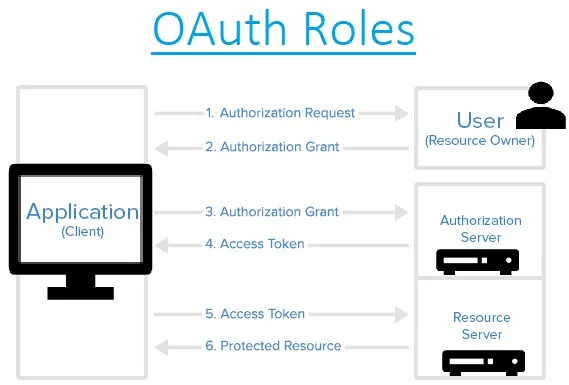
\includegraphics[width=0.7\textwidth]{figures/OAuth_abstract_flow.png}
    \caption{Abstraktní průběh protokolu}%\cite{https://medium.com/@greekykhs/ro-acd8cb4cc0f4#:~:text=OAuth%202.0%20defines%20four%20roles,Resource%20Server%20and%20Authorization%20Server.}} TODO 
    \label{fig:Oauth_roles_diagram}
\end{figure}


\subsection{Grant type: Authorization code}
Jedná se o nejčastěji používanou metodu, především z důvodu optimalizace pro stranu serveru. Autorizační server zde vrací autorizační kód na jedno použití, který je pak vyměněn za přístupový token, podobně jako když se uživatelé přihlašují do webových aplikací s jejich Facebook nebo Google účtem.

\begin{figure}[ht]
    \centering
    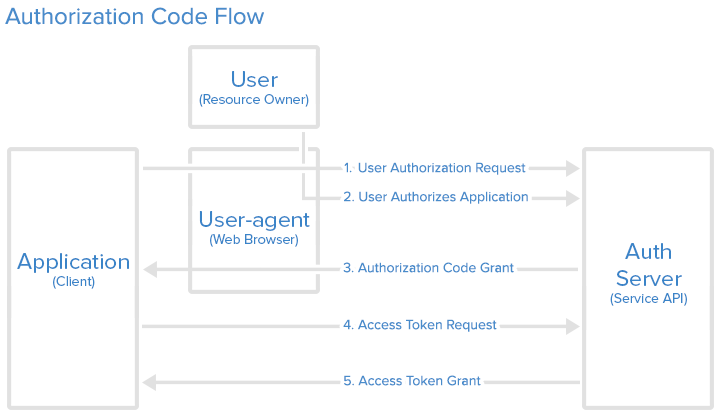
\includegraphics[width=\textwidth]{figures/OAuth_code_flow.png}
    \caption[short]{Průběh autorizace pomocí autorizačního kódu}%TODO https://www.digitalocean.com/community/tutorials/an-introduction-to-oauth-2
    \label{fig:Oauth_auth_flow}
\end{figure}


Na obrázku \ref{fig:Oauth_auth_flow} je popsán průběh výměny autorizačního kódu. 

// todo refactor this
Nejdříve je uživateli poskytnut autorizační URL. Zde se musí přihlásit do přihlašovací služby. Poté potvrdí či zamítnou aplikaci přístup k jejich účtu. Aplikace poté obdrží autorizační kód třeba přes query param %(TODO query param \verb|\ref{desc:query_param}|) 
v URL. Aplikace poté požádá o přístupový token s dalšími autentizačními detaily. A nakonec aplikace dostane přístupový token \textit{případně obnovovací token} pokud autorizace je validní.


\section{Shrnutí}
Jako nejvhodnější styl zabezpečení pro modelovou hru se zdá být API klíč, a to z důvodu jeho jednoduchosti na implementaci, i přes to, že v případě, kdy se uživatelé přihlašují, je vhodný také OAuth2. Z časových důvodů a kvůli nízké škále uživatelských privilegií (administátor, který bude používat backoffice s přímým přístupem na databázi, a uživatelé, kteří budou hru hrát) jsme vybrali právě API klíč. // TODO možná JWT ještě nevíme.


\chapter{Analýza}\label{ch:analysis}
V této kapitole bude probrána specifikace, požadavky na API a také požadavky na celkové fungování hry. Část je také věnována analýze již existujících herních API.

Cílem této práce je vytvořit zdokumentované jednotné API, které bude používáno jak uživatelským prostředím, tak i administrátorským rozhraním.

\section{Analýza již existujících herních API}\label{sec:existing_apis}

Tato část se věnuje představení již existujících online her s evolucí herních situací, která se ukládá mezi sezeními. Těchto her ovšem není mnoho -- většina webových online her nenutí uživatele k přihlášení a také nepodporuje postup či evoluce situací. Takovéto prémiové hry mívají většinou spíše formu desktopových aplikací a v takovém případě by se bohužel špatně analyzovala odcházející a přicházející komunikace.
Byla mi ovšem doporučena jedna hra, která je vytvořená přímo pro hraní za pomocí API, proto jsem se rozhodl tuto hru analyzovat a zjistit, jaké funkce a požadavky by mělo API pro tuto hru splňovat.

\subsection{SpaceTraders API}\label{sub:SpaceTraders}
SpaceTraders je hra založená na REST API, ve které hráči kontrolují a rozšiřují své flotily vesmírných lodí a za jejich pomocí objevují, obchodují a probíjí si vlastní cestu skrz galaxii. Hra je určena pro nadšence, kteří jsou vybízeni vytvořit si vlastní frontend a případně herní mechaniky automatizovat přes jakýkoli jazyk, což může sloužit i jako příjemný nástoj, jak se naučit práci s API nebo nový programovací jazyk. API je zdokumentováno za pomocí technologií OpenAPI a \gls{stoplight}. \cite[]{spacetraders}

Pro dotazování hra využívá jak parametrů dotazu tak proměnných v dotazované URL\@.

Token se vkládá do hlavičky ve formátu \texttt{'Authorization: Bearer INSERT\_TOKEN\_HERE'}. Tento token má formu zakódovaného JWT \sectionref{sec:jwt} objektu pomocí kódování RS256.
Jeho dekódovaný text je zobrazen na obrázku \ref{fig:jwt_spacetraders}.

\begin{figure}[!ht]
    \centering
    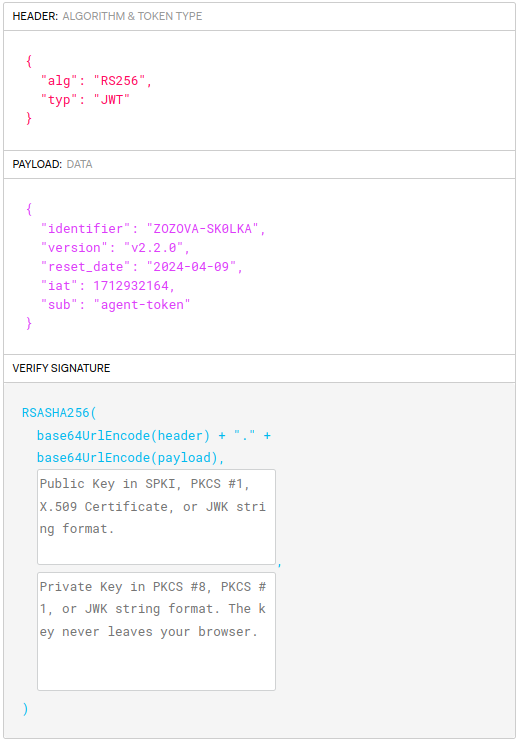
\includegraphics[width=0.5\textwidth]{figures/spaceTraders/jwt.png}
    \caption{Dekódovaný token ze hry SpaceTraders \cite[]{jwt_decoder}}
    \label{fig:jwt_spacetraders}
\end{figure}

Hra nejprve vyžaduje registraci přes endpoint \texttt{/v2/register}. Ten vrátí údaje o novém agentovi spolu s autentizačním tokenem \coderef{code:space_login}[, řádek 3], se kterým se uživatel bude dále ověřovat ve všech následujících požadavcích.

\begin{listing}[!ht]
    \inputminted[breaklines]{json}{resources/code/spaceTraders/login.jsonc}
    \caption{Odpověď na požadavek na registraci\protect\footnotemark}
    \label{code:space_login}
\end{listing}
\footnotetext{Velká část dat musela být pro přehlednost smazána}

Jako odpověď se zde používá formát JSON, který obsahuje především objekt \texttt{data} a poté dodatečné objekty jako třeba \texttt{meta}, ve kterých mohou být další informace jako stránkování. % TODO odkaz na stránkování
Status je použit v souladu s klasickým výkladem statusových kódů % TODO odkaz na ty pravidla někde v restku
a dále je obsahu rozšířen o konkrétní popis chyby v daném požadavku. Příklad je vidět na výpisu \ref{code:space_error}, kde je zobrazena chyba při požadavku na odlet na jinou planetu, neboť loď není na orbitě.


\begin{listing}[ht!]
    \inputminted[breaklines]{json}{resources/code/spaceTraders/error_response.jsonc}
    \caption{Výpis chyby při požadavku odletět na jinou planetu}
    \label{code:space_error}
\end{listing}

\section{Specifikace požadavků}
Pomocí výše provedené analýzy API existujících her, vyčlenění požadavků na funkcionality hry ze strany ostatních členů týmu a za pomocí analýzy dostupných nástrojů pro tvorbu API byly vytyčeny požadavky a funkce, které by mělo API modelové hry podporovat. Jedná se především o CRUD operace se základními objekty, jejich filtrování, stránkování a lazy load. API by taktéž mělo podporovat přihlašování a obranu před základními typy útoků jako je SQL injection, DDOS a DOS útok nebo neoprávněný přístup díky chybám v API.

API by taktéž mělo podporovat validaci všech vstupních dat (rozsahy vstupních hodnot, filtrace speciálních znaků, kontrola správného postupu operací při hraní hry) a mělo by mít odpovídající koncové body pro samotné hraní hry.

\subsection{Funkční požadavky}
Nyní si představíme funkční požadavky na API, které předložili ostatní členové týmu. Tyto požadavky se měnily a rozšiřovaly spolu s průběhem návrhu i implementace. Některé požadavky, které vzešly primárně z backoffice se využívají ve frontendu a případně i naopak.

\subsubsection*{Požadavky, které byly vyčleněny primárně ze strany backoffice}

\begin{enumerate}[label=\textbf{F\arabic*}:, leftmargin=*, align=left]
    \item \textbf{CRUD operace} -- Nad základními objekty, se kterými se bude často pracovat, a upravovat pomocí endpointů. Těmito objekty jsou \texttt{akce, efekty, předměty, charaktery a jejich vlastnosti, dobrodružství, kampaň, obchody, nepřátelé, překážky, lokace} a \texttt{části lokace}
    \item \textbf{Filtrování} -- Možnost vyhledat objekty podle vstupních parametrů u koncových bodů, které poskytují seznam objektů.
    \item \textbf{Lazy load} -- Způsob načítání dat, který umožňuje vracet pouze daný objekt bez jeho závislostí, případně vrácení pouze těch závislostí, které se určí. Výsledkem je rychlejší zpracování a menší objem přesunutých dat, když uživatel tyto závislosti nepotřebuje. Namísto objektu se tedy vrátí jen jeho identifikátor.
    \item \textbf{Stránkování} -- Další způsob předávání dat, který umožní jejich postupné zpracování, což vede ke zkrácení času potřebného k vyhodnocení požadavku jak v API tak ve zobrazovací části.
    \item \textbf{Caching} -- Již jednou zpracovaná data z databáze není třeba znovu získávat z databáze, pokud nedošlo ke změně. Tato funkcionalita umožní násobně rychlejší odezvu pro opakované získávání stejných dat.
    \item \textbf{Administrátorská práva} -- Ne všichni mohou mít přístup pro úpravu dat v databázi. Díky administrátorským přihlašovacím údajům a následnému tokenu se budou moci upravovat a vkládat data do databáze pouze s odpovídajícím ověřením.
    \item \textbf{Validace} -- Data vkládaná do databáze budou validována a případně vrátí chybovou hlášku, podle které bude možno snadno identifikovat chybu vstupních dat a následně ji opravit.
\end{enumerate}


\subsubsection*{Požadavky primárně ze strany uživatelského prostředí}

\begin{enumerate}[label=\textbf{F\arabic*}:, leftmargin=*, align=left]
    \item \textbf{Získávání objektů} -- Bude umožněno získávat jakékoliv objekty, které neobsahují herní data či jiné citlivé informace, přímo z databáze.
    \item \textbf{Podpora herního průběhu} -- Uživatel bude moci projít celým soubojem a interagovat s entitami v něm za pomocí řady validovaných a přehledně uspořádaných koncových bodů.
    \item \textbf{Zamezení zneužití} -- Postup operací v herním průběhu bude kontrolován tak, aby se zamezilo případnému zneužití nebo obcházení pravidel hry.
    \item \textbf{Přihlášení} -- Uživatel se bude moci přihlásit a získat token pro ověření v dalších požadavcích.
    \item \textbf{Herní data} -- Uživatel bude mít pod svým účtem uložený postup hry a bude moci pokračovat tam, kde skončil. Dále bude mít možnost vytvářet nové postavy pro kampaně a také nová dobrodružství.
    \item \textbf{Validace} -- Obsah vstupních dat bude validován a případně vrátí smysluplnou chybovou hlášku.
    \item \textbf{Obrázky} -- Bude možné získat obrázek z url adresy přiložené k objektu, případně v požadavku specifikovat jeho velikost.
\end{enumerate}



\subsection{Nefunkční požadavky}
Dále je důležité vyhradit si nefunkční požadavky. Jejich vznik je stejný jako požadavky funkční, byly sestrojovány postupně s vývojem na základě zkušeností a požadavků ostatních členů týmu.


\begin{enumerate}[label=\textbf{F\arabic*}:, leftmargin=*, align=left]
    \item \textbf{Rozdělení API na dvě části} -- Z důvodu spolupráce na API s jinými členy týmu, především herním systémem, který pro svůj chod využívá stejných modelů, bylo rozhodnuto, že herní logika i mapování bude v jednom projektu. Tomu tedy musí být přizpůsobena i spolupráce a podpůrné technologie.
    \item \textbf{Dokumentace} API bude zdokumentováno za pomocí OpenAPI a pro vizuální zobrazení koncových bodů bude použit Swagger, který zároveň poslouží jako skvělé ladící rozhraní.
    \item \textbf{Hosting} API bude stejně jako ostatní části projektu hostováno na veřejných serverech.
    \item \textbf{Přehlednost} Koncové body API by měly být samopopisující a snadno pochopitelné.
    \item \textbf{Standardizovanost} API se bude držet ověřených dobrých praktik z praxe a bude udržovat jednotnost a standardizovanost.
\end{enumerate}

\section{Uložení dat}\label{sec:data_storage}
Pro ukládání dat existuje mnoho různých databázových systémů, ať už relační nebo dokumentové. v této kapitole budou probrány možnosti výběru databáze pro hru.

\subsection{SQL database}\label{sec:data_storage:relational_db}
Relační databáze, jindy nazývané \gls{sql} databáze, jsou databáze, které využívají strukturovaných dotazů (\gls{sql}) pro manipulaci dat. Data jsou reprezentována tabulkami, které mají předdefinovány relace mezi ostatními tabulkami. Je to nejčastěji používaný styl databáze. Nejlépe se hodí pro strukturovaná data. Jedny z nejpoužívanějších relačních databází jsou \textbf{MySQL}, \textbf{PostgreSQL} a \textbf{SQLite}.\cite{guidetochoosingdatabase}\cite{howtochoosedatabase}

Při použití \gls{rdbms} chráníme svá data před ztrátou a díky ACID vlastnostem máme jistotu o konzistenci dat. Nyní níže budou popsány jednotlivé vlastnosti ACID.\label{sec:data_storage:relational_db:ACID}\cite{acidvsbase}

\textbf{Atomičnost} zajišťuje, že se všemi transakcemi je zacházeno jako s jedním celkem. Jediné dvě možnosti jak transakce může dopadnout je buď celá úspěšně a nebo celá neúspěšně. Když se transakce skládá z více částí, majoritní část se provede tak provedené operace v transakci se vrátí do původní podoby.

Díky \textbf{konzistenci} budou do databáze vložena pouze validní data. Pokud vstupní data nejsou validní, databáze se vrátí do původní podoby. Díky tomu se předejde poškození databáze.

\textbf{Izolace}  zajišťuje, že nedokončené transakce nebudou ovlivněny jinými transakcemi. Díky této vlastnosti může jednoduše pracovat na databázi více uživatelů najednou bez ovlivnění se navzájem.

\textbf{Durabilita} znamená, že uložená data nebudou ztracena ani když transakce selže nebo když dojde k výpadku systému.

Mezi hlavní nevýhody relačních databází je nízká flexibilita neboli neefektivnost pracovat s nestrukturovanými daty, takže se nedají dobře použít na Internet of Things aplikace. S neflexibilitou se pojí špatný návrh pro komplexní datové struktury. Taky relační databáze se nemohou škálovat do šířky, neboli zátěž se nemůže rozložit na více serverů.

\subsection{noSQL database}\label{sec:data_storage:document_db}
Dokumentové databáze umožňují ukládání a zpracovávání nestrukturovaných dat (hudba, fotografie, atd.), což umožňuje vývojářům mít větší flexibilitu nad daty, což je jedna z největších výhod dokumentových databází. Taktéž se mohou škálovat do šířky, takže zpracování velkého množství dat není obtížné. Mají taktéž velkou toleranci proti chybám. S velkou tolerancí chyb se pojí limitované ACID vlastnosti, kdy místo ACID využívají BASE vlastnosti, které jsou popsány níže. Tyto databáze nemají unifikovaný dotazovací jazyk jako relační databáze a mohou mít problém s komplexními dotazy. Nejčastěji používané dokumentové databáze jsou \textbf{MongoDB} a \textbf{CouchDB}.\cite{guidetochoosingdatabase}\cite{howtochoosedatabase}

\textbf{BASE}\label{sec:data_storage:base} je zkratka pro \textbf{Basically Available}, což znamená že databáze bude dostupná pro uživatele za všech okolností. neboli uživatel nemusí čekat než jiný uživatel dokončí svou transakci. \textbf{Soft state} znamená, že data se mohou nacházet v temporálním stavu když běží více transakcí zároveň a můžou se změnit i po dokončení transakce. Data přejdou do finálního stavu až když jsou všechny transakce dokončeny. S tím se pojí \textbf{Eventually consistent}, kdy data se dostanou do konzistentního stavu po všech souběžných aktualizacích. V tento moment všechny aplikace vidí stejná data.\cite{acidvsbase}

\subsection{Porovnání SQL a noSQL databází}

V tabulce \ref{tab:sql_vs_nosql} máme přehledně porovnány vlastnosti SQL a noSQL databází. Pro naše použití jsme vybrali že bude vhodnější SQL databáze díky reprezentaci jedna tabulka v databázi = jeden objekt v API. Taktéž jsme všichni již pracovali s SQL databázemi a vedoucím práce nám byla doporučena SQL databáze. Přechod na noSQL by bylo zabředávání do neznámých vod.

\begin{table}
    \centering
    \begin{tabular}{|l|l|l|}
        \hline
        kritérium        & SQL               & noSQL            \\
        \hline
        Typ dat          & Strukturovaná     & Nestrukturovaná  \\
        Flexibilita      & Nízká             & Vysoká           \\
        Škálovatelnost   & Vertikální        & Horizontální     \\
        Schéma           & Striktní          & Dynamické        \\
        Transakce        & ACID              & BASE             \\
        Dotazovací jazyk & SQL               & Není unifikovaný \\
        Příklady DB      & PostgreSQL, MySQL & MongoDB, Redis   \\
    \end{tabular}
    \caption{Porovnání SQL a noSQL databází}\label{tab:sql_vs_nosql}
\end{table}

Nyní si představíme nejznámější SQL databáze.

\subsection{MySQL}\label{sec:data_storage:mysql}
MySQL je jedna z nejpoužívanějších databází. Má velkou podporu a je open-source, funguje velmi dobře s většinou knihoven a frameworků. Skvěle se hodí na menší až střední projekty. Obsahuje komplexní sadu funkcionalit jako jsou triggery, procedury, pohledy a podpora transakcí. Ve větších projektech může mít problémy s výkonem  a s komplexními dotazy.\cite{guidetochoosingdatabase}\cite{howtochoosedatabase}


\subsection{PostgreSQL}\label{sec:data_storage:postgresql}
Tato databáze je objektově relační což je podobné jako relační jen data jsou ukládány v objektech místo tabulek jako je tomu například u MySQL. Přednosti PostgreSQL jsou pokročilé indexování, vlastní datové typy , komplexní dotazy a cizí klíče, a dovoluje volat procedury napsané v jiném jazyce než SQL. Nicméně je náročnější na výkon, některé vlastnosti mohou být náročné na nakonfigurování a může být pomalejší při čtení dat.\cite{guidetochoosingdatabase}\cite{howtochoosedatabase}

\subsection{Výběr databáze}
Nakonec jsme vybrali primárně díky doporučení našeho vedoucího práce MariaDB, což je založeno na MySQL. MariaDB je osamocená větev původních vývojářů, po tom co MySQL bylo získáno společností Oracle. Je rychlejší, podporuje \textit{neviditelné sloupce} a má propracovanější views.

\section{Technologie pro tvorbu API}\label{sec:api_technologies}
v této kapitole bude probráno jaké frameworky a technologie jsou dostupné pro tvorbu API. Níže je výčet těch nejznámějších a nejpoužívanějších s ohledem na požadavky a zkušenosti týmu.

\subsection{Spring Boot}\label{sec:api_technologies:spring}
\begin{wrapfigure}{r}{0.3\textwidth} % TODO idk jestli tu dávat obrázky
    \centering
    
\includegraphics[width=0.2\textwidth]{figures/logos/springboot.png}
    \caption{Logo Spring Bootu, zdroj: } %%TODO kdyžtak to dát do cite \url{https://www.pngaaa.com/detail/2459546}
    \label{fig:spring}
\end{wrapfigure}
Založen originálně na Spring technologii ale snaží se udělat originální Spring framework více uživatelsky přívětivý. Spring boot obsahuje v sobě vše, co je třeba, bez velkého konfigurování knihoven. Je určen i pro velké aplikace ve velkých společnostech jako je Netflix. Kromě programovacího jazyku Java podporuje i Kotlin a Groovy. Má velkou podporu komunity a skvělou dokumentaci. Ovšem může být náročnější na hardware a binární soubory jsou větší kvůli velkému množství knihoven.

\subsection{ASP.NET Core}\label{sec:api_technologies:asp}
Uzavřený framework od Microsoftu, který je určen pro webové aplikace. Jedná se o alternativu ke Springu u Javy ovšem pro jazyk C\#. Je zde navíc lepší podpora asynchronních operací a je zde \gls{linq}. Oproti Springbootu má i vlastní ekosystém nástrojů jako je třeba microsoft Azure nebo MSSql databáze. ASP.NET Core i Spring boot jsou velmi solidní frameworky i pro velké firmy a vyloženě záleží na preferenci programovacího jazyka.

\subsection{Django REST}\label{sec:api_technologies:django}
Založeno na Django frameworku a jeho pohledech založených na třídách \textit{class-based views}. Celkově se jedná o velice bezpečný framework určený pro programovací jazyk Python, s rychlou učící křivkou a s obsáhlou dokumentací. Ovšem u větších projektů je méně přehledný než výše zmíněné frameworky.

\subsection{Fast API}\label{sec:api_technologies:fast}
Jakožto alternativu k Djangu zde máme Fast API, kde je plně podporováno asynchronní programování a je přímo určeno pro vývoj RESTful API. Je taktéž pro Python, je velmi rychlý jak na naučení tak i framework jako takový a je plně otypovaný oproti Djangu. Má dobrou dokumentaci a mezi vývojáři je čím dál populárnější. Ovšem má horší validaci vstupních dat.


\subsection{Výběr frameworku}\label{sec:api_technologies:summary}
Pro účely RESTful API byl výběr očividný, Fast API které je navrhnuto pro rychlou tvorbu RESTful API a pro vývojáře velice příjemným otypováním. Je taktéž jeden z nejrychlejších Python frameworků v některých věcech na úrovní například Spring bootu.\cite{benchmarks} Taktéž Python je jeden z jednodušších jazyků a všichni členové týmu už s ním mají zkušenosti. Ovšem později se na doporučení přešlo na Spring boot díky jeho jednoduššímu \gls{orm} a větší přehlednosti.
\chapter{Návrh}\label{chap:design}
Tato kapitola se bude zabývat návrhem sestavy technologií, které se budou využívat pro realizaci \gls{api}.

\section{Model vývoje}\label{sec:development_model}
Jako model vývoje byl použit klasický vodopádový model \figureref{fig:waterfall}, který sice v praxi není úplně realistický, ale je dobrým základem pro popis vývojového procesu modelové hry. Používá se primárně v situacích, kdy je definice projektu jasná a je zřejmý i cíl, kdy je dost času pro vývoj a kdy je možné všechny fáze vývoje pečlivě naplánovat, aby se minimalizovaly chyby.

První vlastností tohoto modelu je \textbf{sekvenční přístup}, neboť nemožnost pracovat na další části vývoje, dokud přechozí není plně dokončena. Další z vlastností je \textbf{řízení dokumentací}, kdy se všechny fáze vývoje musí pečlivě dokumentovat, aby se minimalizoval čas strávený zpětnou analýzou provedených kroků. \textbf{Kontrola kvality} je při tomto modelu důležitá, neboť chyby, které by se mohly vyskytnout v prvotních fázích vývoje, se mohou nepříjemně projevit a vývoj zkomplikovat. S tím se pojí i \textbf{přísné plánování}, kdy je nutné všechny fáze vývoje pečlivě naplánovat a zvážit možná rizika, která by mohla vzniknout.

Tímto modelem jsme se snažili řídit, ale i přes důkladné promyšlení použitých návrhů se muselo v průběhu pár drobností upravovat. 

\begin{figure}[!ht]
    \centering
    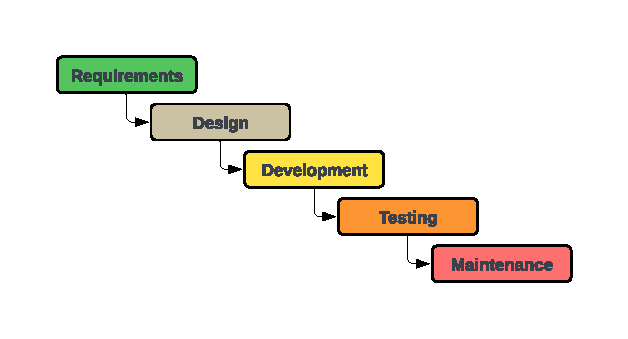
\includegraphics[width=0.8\textwidth]{figures/impl/API Implementation - waterfall model.pdf}
    \caption{Vodopádový model vývoje}\label{fig:waterfall}
\end{figure}

Ve fázi \textbf{požadavků} byly vzneseny nápady, jak samotná hra bude fungovat, jaké mechaniky použijeme a jakým způsobem by je bylo možné implementovat, přičemž nám vystačil pouze dokument s nápady a požadavky. Taktéž si zde všichni ujasnili, jaké herní mechaniky budou použity a za jakých okolností. 

Ve druhé fázi \textbf{návrhu} probíhala tvorba upřesňujících diagramů, návrhu architektury a uživatelského rozhraní. V našem případě byly přesněji rozvrženy jednotlivé mechaniky a bylo blíže popsáno, co se od nich očekává. Zároveň byly aplikovány návrhové vzory, které byly vhodné pro daný problém, především ty týkající se RESTful API.

Fáze \textbf{vývoje} zahrnuje implementaci návrhů a vytvoření funkčního programu. V této fázi se taktéž využívají unit testy, které ověřují funkčnost jednotlivých částí programu. 

Poslední fáze, \textbf{testování} a \textbf{údržba}, se starají o to, aby program byl bez chyb a aby jednotlivé programy fungovaly jako celek. Po tom, co byl projekt otestován a vše je funkční, jde do produkčního prostředí a už se pouze udržuje, což zahrnuje opravování drobných chyb, které nebyly odhaleny během testování.

\section{Spolupráce}\label{sec:collaboration}
Jak už několikrát bylo naznačeno, tato práce byla vytvářena v týmu, kde měl každý člen na starosti jinou hlavní komponentu.
\begin{itemize}[itemsep=0pt,parsep=0pt]
    \item \textbf{Herní systém} -- Barbora Kovalská
    \item \textbf{Backoffice} -- Pavel Mikula
    \item \textbf{Frontend} -- Miroslav Osoba
    \item \textbf{API} -- Martin Korotwitschka
\end{itemize}

V průběhu bylo třeba přidat i jiné komponenty, protože bez nich by nebylo zprovoznění hry jakožto celku možné, takže zvlášť na nich pracovalo více členů týmu. V raných fázích vývoje bylo taktéž běžné, že se jednotliví členové více podíleli i na ostatních úkonech. 

Komunikace v prvotních fázích vývoje probíhala především za pomocí nástroje Github Issues. Později, když už byla kostra projektu funkční, stačila interní komunikace.

\subsection{Rozdělení práce}\label{sec:collaboration:job_distribution}
Jak lze vidět na Obrázku \ref{fig:job_distribution}, každý člen týmu nesl zodpovědnost za svou část projektu. Toto rozdělení vycházelo především ze zadání prací. 

\begin{figure}[h]
    \centering
    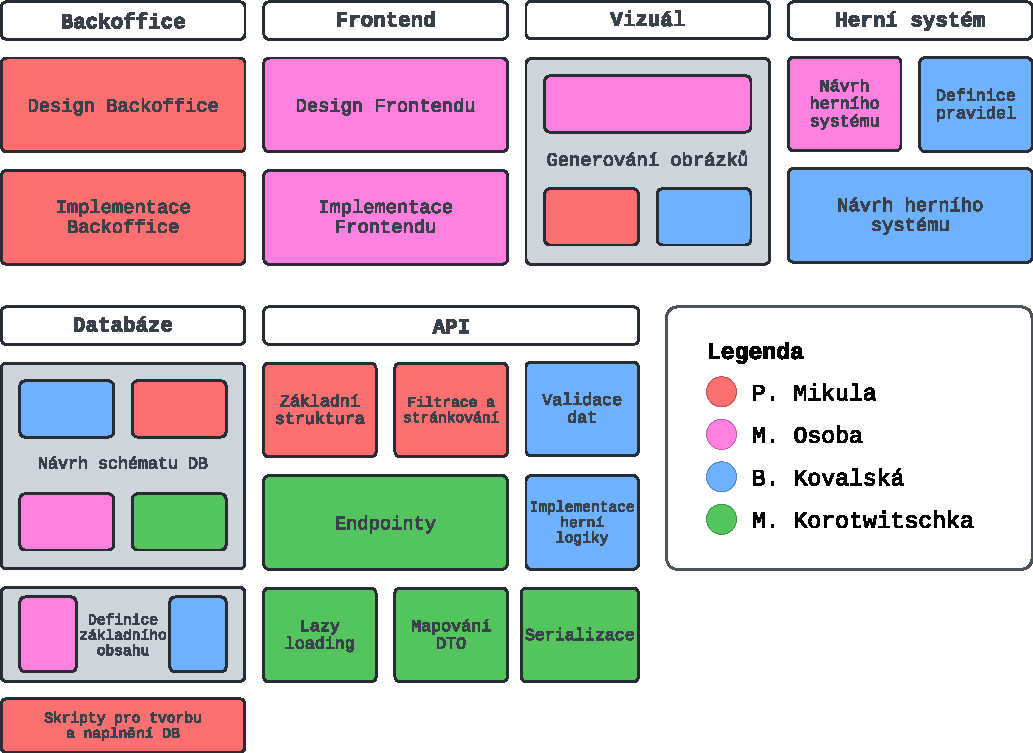
\includegraphics[width=\textwidth]{../../shared/diagrams/blocks.pdf}
    \caption{Rozložení práce v týmu}
    \label{fig:job_distribution}
\end{figure}

Pro přehlednost a verzování kódu byla vytvořena organizace na platformě GitHub \figureref{fig:gitOrg}, kde se vytvořily samostatné repozitáře pro každou část projektu. Taktéž se zde vedly \textit{Issues}, které zvlášť v prvotních fázích ulehčovaly vývoj a komunikaci.

\begin{figure}[H]
    \centering
    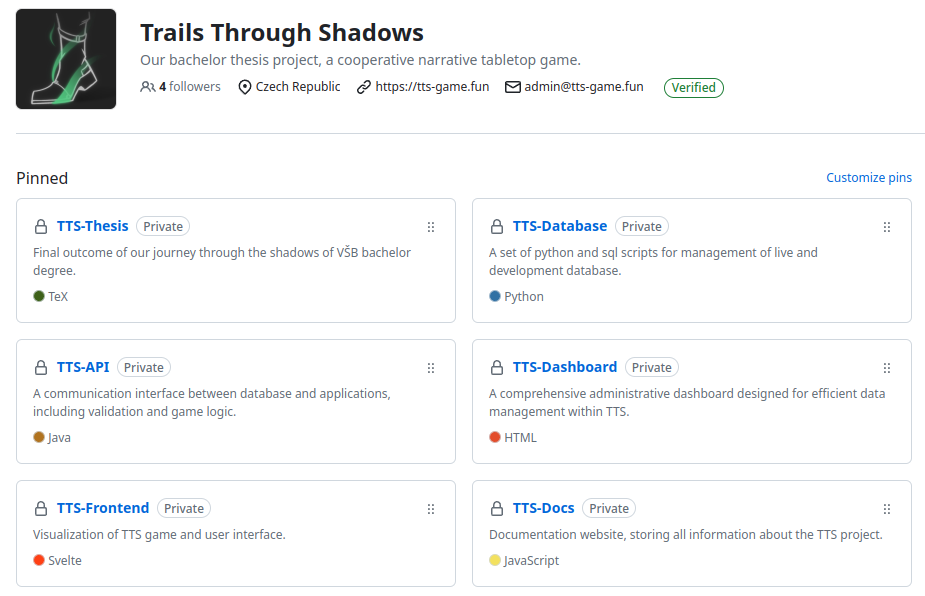
\includegraphics[width=\textwidth]{../../shared/figures/gitOrg.png}
    \caption{Organizace \textit{Trails Through Shadows} na platformě GitHub}
    \label{fig:gitOrg}
\end{figure}

Verzovací systém byl potřeba obzvlášť v případě API, na kterém pracovali primárně dva členové týmu. K ulehčení spolupráce zde bylo využito tzv. větví pro implementaci rozličných funkcionalit. Dokud nebyla kostra API hotová, nebylo takovéto rozdělování účinné a často se tak musely řešit konflikty.

Poté, co byla vytvořena kostra API, se začaly řádně využívat větve a jejich pravidla. Jako hlavní větev byla zvolena \textit{master}, na které byla vždy poslední stabilní verze, která byla nasazena na server. Další větev byla \textit{development}, na které se uchovávaly většinou funkční ale neotestované funkcionality. Ostatní větve se už v pozdější fázi vývoje nevyužívaly, protože každý vývojář pracující na tomto projektu měl svou vlastní složku, ve které pracoval, čímž bylo zabráněno konfliktům. Výše popsané strategii dělání větví a jejich následnému sloučení se říká \textit{Gitflow}.

\begin{figure}[H]
    \centering
    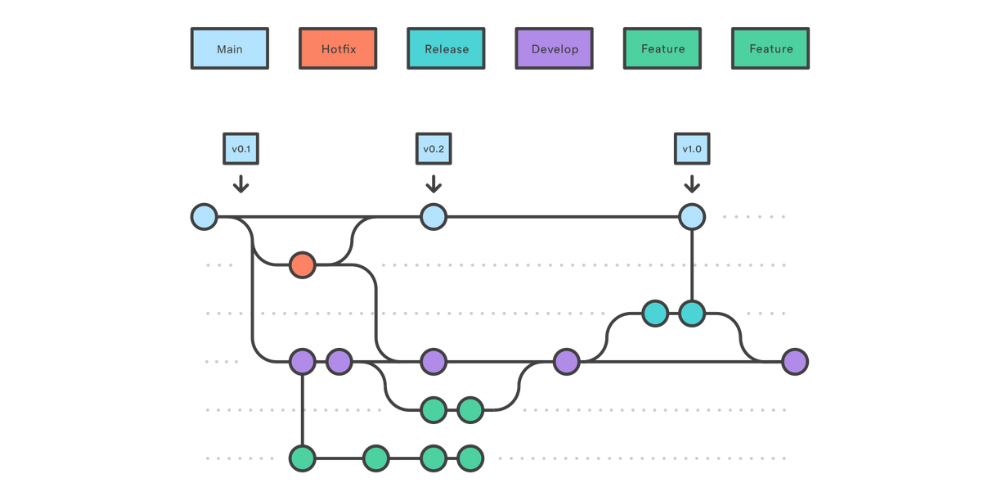
\includegraphics[width=\textwidth]{figures/impl/git-flow.png}
    \caption{Příklad \textit{Gitflow} workflow}
    \label{fig:gitflow}
\end{figure}

U repozitáře TTS-Thesis, kde byly uchovány texty všech našich prací, jsme používali Trunk-Based vývoj, kde se všechny akce se provádějí na hlavní větvi. Tento styl fungoval hlavně díky tomu, že každý měl svou vlastní složku, jejíž funkčnost nebyla na těch ostatních vůbec závislá. Díky tomu jsme mohli mít instantní nasazení vytvořeného PDF z \LaTeX ~souborů na webovou stránku.


\section{Databáze}\label{sec:database}
Návrh celého projektu byl započat vytvořením návrhu databáze. Na návrhu se podíleli všichni členové týmu \figureref{fig:job_distribution}, jelikož bylo nutné, aby všichni členové věděli, co a jak bude v databázi strukturované. Návrh probíhal za pomocí placeného nástroje \textit{dbdiagram.io}, kde se  všichni mohli podílet i online na tvorbě schématu v jeden časový moment. Tento nástroj taktéž podporuje export do řady SQL dialektů, mimo jiné i do MySQL, který jsme použili, protože databáze MariaDB používá stejnou syntaxi \sectionref{sec:data_storage}.

V kompletním ER diagramu databáze \figureref{fig:dix:database_schema} lze vidět jednotlivé rozdělení tabulek dle barvy do jednotlivých logických celků \figureref{fig:database_schema:block}[, zjedodušené blokové schéma]. Každá tabulka má v prvním sloupci zaznamenáno, zda se jedná o klíč, v druhém název atributu a ve třetím jeho datový typ. Z jednotlivých řádků je vidět závislost na ostatních tabulkách.

\begin{figure}[h]
    \centering
    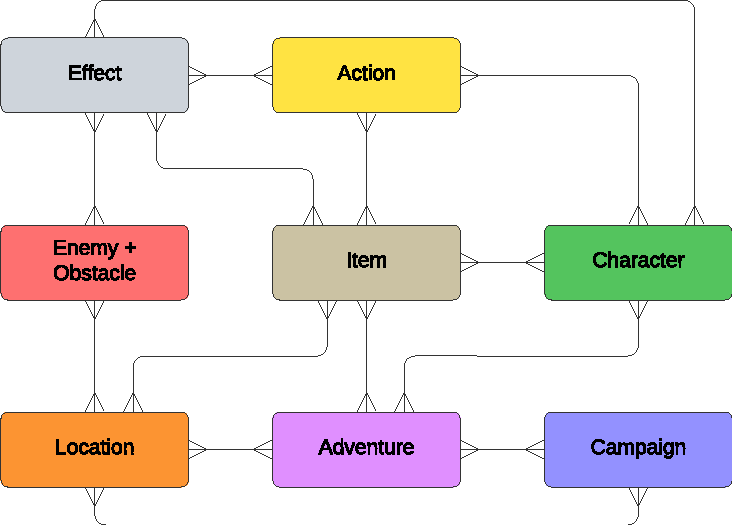
\includegraphics[width=0.5\textwidth]{../../shared/diagrams/er_macro.pdf}
    \caption{Zjednodušené databázové schéma podle logických celků}
    \label{fig:database_schema:block}
\end{figure}

Na prvním místě je žlutá sekce, která pojednává o \textbf{Akcích}. Základem je tabulka Action, která specifikuje, o jakou akci se jedná, zda o \textit{útok, pohyb, dovednost, obnovení karet} nebo o \textit{přivolání poskoka}. Akce samozřejmě může mít i více typů, a skoro každý typ akce může mít nějaký přídavný efekt.

Šedá sekce \textbf{Efekt} přidává spoustu modifikací, ať už jakékoli postavě jako například \textit{rezistenci na otrávení}, nebo modifikaci k útoku jako třeba \textit{krvácení}.

Zelená sekce se stará o \textbf{Postavu hráče}. Jako hlavní tabulka je zde \textit{Character}, která má vazbu na definici, o jakou postavu se bude jednat, neboli tabulky \textit{Třída} a \textit{Rasa}, podle kterých postava dostane své \textit{Akce}. Hráč má i inventář, ve kterém může mít jednotlivé předměty, které mu přidávají ať už statické bonusy nebo jednorázové výhody v boji.

Béžová sekce \textbf{Předmět} má na starosti \textit{Předměty} a jejich vazby na obchody, ve kterých se nacházejí. Předměty, jak již bylo zmíněno výše, přidávají hráči bonusy.

\textbf{Protivník a Překážka} jsou v červené sekci a specifikují protivníka nebo překážku v lokaci, ve které se bude bojovat. Jsou spojeny stejnou barvou, protože tyto dvě entity jsou si velice podobné, rozdíl je jen v tom, že jedna je dynamická a druhá statická.

Sekce \textbf{Lokace}, která je oranžová, specifikuje lokaci, na které bude probíhat bojová interakce. Základem je tabulka \textit{Location} která má relace na vstupní a výstupní hexagony, na protivníky a překážky, dveře a na části, ze kterých se tato lokace skládá. 

Jako poslední sekce je \textbf{Kampaň a Dobrodružství}, které spolu úzce souvisí, i přes to, že jsou zapsány jinou barvou (Kampaň modrá a Dobrodružství fialová). \textit{Kampaň} má příběh k dané lokaci, seznam \textit{dobrodružství} a seznam lokací, které jsou v rámci ní propojené. \textit{Dobrodružství} má seznam hráčů, kteří se účastní a seznam dostupných lokací.

\chapter{Implementace}\label{chap:implementation}

\section{Implementace API}\label{sec:impl:api}
Implementace původně probíhala ve \gls{framework}u FastAPI \sectionref{sec:api_technologies:fast}, ale po zjištění složitosti ORM při použití Python knihovny SQL Alchemy bylo doporučeno jedním z řešitelů (P. Mikula), použít raději Javu a její \gls{framework} Spring Boot, za použití knihoven jako je JPA, Lombok, Jackson a jiných. Tato změna nebyla obtížná, jelikož vývoj byl teprve ve velice rané fázi vývoje. Taktéž Spring Boot byl jeden z kandidátů.

Nyní budou popsány nejdůležitější knihovny \gls{framework}u Spring Boot, které byly použity při implementaci \gls{api}.


\subsection{Knihovny Spring Boot}\label{sec:impl:spring}
% TODO nějaký lepší název nebo něco

Tyto knihovny jsou základním stavebním kamenem jak pro samotné koncové body tak pro \gls{orm}. Na obrázku \ref{fig:JPA} máme vizuální schéma toho, jak tyto knihovny spolu fungují.

\begin{figure}[ht!]
    \centering
    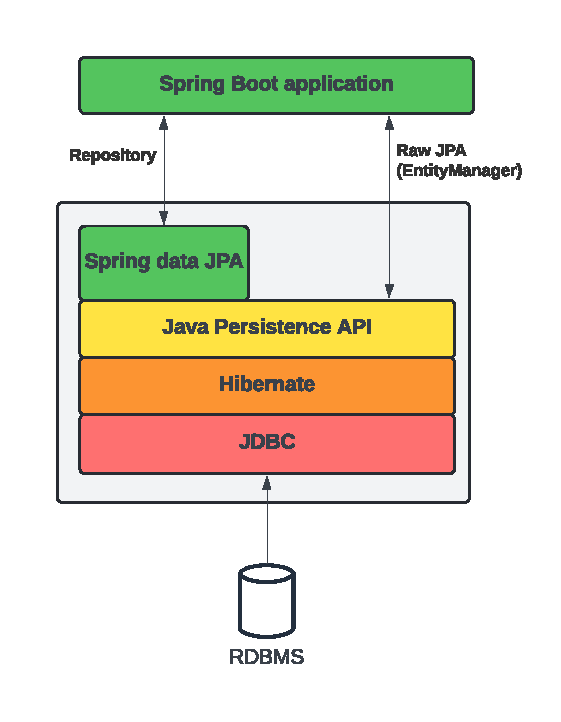
\includegraphics[width=0.5\textwidth]{figures/impl/API Implementation - JPA.pdf}
    \caption{Struktura Spring Boot Data JPA aplikace}
    \label{fig:JPA}
\end{figure}

\subsubsection*{Spring Data JPA} \label{sec:impl:spring:data:jpa}
JPA neboli Java Persistence API je jedna ze součástí Spring Data Family, která umožňuje jednoduché implementování \textbf{repozitářů} založených na JPA a signifikantně zjednodušuje implementaci datové vrstvy aplikace. Umožňuje používat základní SQL požadavky a ORM bez námahy vytvoření vlastních požadavků. V ukázce na výpisu \ref{code:JPA_repo} je vidět implementace repozitáře pro entitu \textit{Enemy}. Zde jsou již naimplementované základní metody jako \textit{save}, \textit{findAll}, a je zde navíc metoda \textit{findAllByLocationId} s vlastním SQL dotazem.

\begin{listing}[ht!]
    \inputminted[]{Java}{resources/code/impl/EnemyRepo.java}
    \caption{Ukázka JPA repozitáře}
    \label{code:JPA_repo}
\end{listing}

\subsubsection*{JPA}
Spring Data JPA používá několik dalších knihoven a dalo by se říci, že to je jakýsi zprostředkovatel nad \textbf{JPA}. JPA zajišťuje objektově relační mapování (\gls{orm}), což usnadňuje práci s ukládáním objektů do databáze a naopak.

Základním objektem v JPA je \textit{Entita}. Ta reprezentuje objekt v databázi, který je poté namapován na jednotlivé vlastnosti třídy \coderef{code:jpa_entity}. Třídu označíme jako entitu pomocí anotace \textit{@Entity} a poté pomocí \texttt{@Table} můžeme upřesnit jméno tabulky, schéma databáze a jiné atributy. Za pomoci anotace \textit{@Id} označíme primární klíč a nebo pomocí \texttt{@EmbeddedId} označíme složený primární klíč. Atributy třídy označíme pomocí \texttt{@Column} kdy ve výchozím stavu atribut může nabývat prázdné hodnoty a sloupec v databázi se jmenuje stejně jako atribut. Relace se mapují pomocí jedné z anotací \texttt{@OneToOne}, \texttt{@OneToMany}, \texttt{@ManyToOne} nebo \texttt{@ManyToMany} podle toho, jakou relaci potřebujeme. V této implementaci probíhal nejdříve návrh databáze, takže jsme používali pouze \texttt{1:N} relace abychom se vyhnuli cyklickým závislostem, protože vazební \texttt{M:N} tabulky již byly v databázi.

\subsubsection*{Hibernate}\label{sec:impl:hibernate}
Jedna z konkrétních implementací JPA je Hibernate. Za pomocí výše zmíněných anotací nebo XML \sectionref{sec:formats:xml} schématu si udržuje schéma databáze a stav objektů, udržuje tedy data perzistentní. Díky schématu databáze Hibernate ví, jak se mají data z databázových tabulek transformovat do objektů a naopak. \cite[]{enwiki:1217225259}

\subsubsection*{JDBC}\label{sec:impl:jdbc}
Neboli Java Database Connectivity je API pro přístup k databázi. Poskytuje metody pro dotazování se na na databázi pomocí \gls{sql} a umožňuje zpracovávat výsledky dotazů.

\begin{listing}[ht!]
    \inputminted[breaklines]{Java}{resources/code/impl/EnemyDTO.java}
    \caption{Příklad entity v JPA}
    \label{code:jpa_entity}
\end{listing}


\subsection{Jiné použité knihovny} %%TODO reformat nadpis aaaaaa
V této kapitole budou popsány knihovny, které nejsou součástí Spring Bootu, ale byly ve větší míře použity při implementaci API.

\subsubsection*{Lombok}\label{sec:impl:lombok}
Lombok je knihovna, která za pomocí anotací automaticky generuje základní repetetivní kódy jako jsou gettery a settery, konstruktory a jiné, což je pro vývojáře velice vítané.

První možností této knihovny jsou anotace \texttt{@Getter} a \texttt{@Setter}, které automaticky vygenerují \textbf{gettery} nebo \textbf{settery} s příslušnými modifikátory přístupu pro daný atribut \coderef{code:lombok:getters}. Tato anotace lze použít i nad celou třídou a automaticky vygeneruje kód pro všechny atributy. Vygenerované metody jsou ukázány na výpisu \ref{code:lombok:getters:generated}.

\begin{listing}[H]
    \begin{minted}[fontsize=\footnotesize]{Java}
        public class GetterSetterExample {
            @Getter private int age = 10;
            @Setter(AccessLevel.PROTECTED) private String name;
        }
     \end{minted}
    \caption{Použití anotací \texttt{@Getter} a \texttt{@Setter}}
    \label{code:lombok:getters}
\end{listing}

\begin{listing}[H]
    \begin{minted}[fontsize=\footnotesize]{Java}
        public class GetterSetterExample {
            private int age = 10;
            private String name;
            public int getAge() {
                return this.age;
            }
            protected void setName(String name) {
                this.name = name;
            }
        }
     \end{minted}
    \caption{vygenerovaný kód za pomocí \texttt{@Getter} a \texttt{@Setter}}
    \label{code:lombok:getters:generated}
\end{listing}

Další důležité anotace se týkají konstruktorů. \texttt{@NoArgsConstructor} vygeneruje prázdný konstruktor, \texttt{@AllArgsConstructor} vygeneruje konstruktor se všemi atributy \coderef{code:lombok:constructor} a jako poslední anotace \texttt{@RequiredArgsConstructor} vygeneruje konstruktor s všemi atributy označenými jako \texttt{@NonNull}. Tato anotace se zapisuje nad třídu. \cite{lombok:constructor}

\begin{listing}[H]
    \begin{minted}[fontsize=\footnotesize]{Java}
        public class ConstrExample {
            private int age;
            private String name;

            ConstrExample(int age, String name) {
                this.age = age;
                this.name = name;
            }
        }
    \end{minted}
    \caption{Příklad kódu vygenerovaného pomocí \texttt{@AllArgsConstructor}}
    \label{code:lombok:constructor}
\end{listing}


Práci si je možné zjednodušit ještě více za pomocí anotace \texttt{@Data}, která vygeneruje výše zmíněné \texttt{@Getter, @Setter, @RequiredArgsConstructor} a navíc \texttt{@ToString} a \texttt{@EqualsAndHashCode}.\cite{lombok:data} Anotace \texttt{@ToString} vygeneruje metodu \texttt{toString()}, která objekt převede na textový řetězec, kde za pomoci různých parametrů můžeme upravovat, které atributy se budou vypisovat a jak. Další anotace, kterou \texttt{@Data} obsahuje, je \texttt{@EqualsAndHashCode}, která vygeneruje metody pro porovnávání objektů.

Za zmínku také stojí anotace \texttt{@Builder}, která vygeneruje interní třídu podle návrhového vzoru Builder\cite{refactoringGuru:builder}, jež slouží k vytváření objektů. \cite{lombok:builder}

\subsubsection*{Jackson}\label{sec:impl:jackson}
Tato knihovna slouží pro serializaci objektů do formátu JSON \chapterref{sec:formats:json} a naopak. S její pomocí bylo možné specifikovat, jak se budou jednotlivé objekty či atributy serializovat, například zde lze nastavit ignorování některých atributů nebo úplně vlastní serializace.

\subsubsection*{Swagger}\label{sec:impl:swagger}
Swagger je open-source dokumentační nástroj pro \gls{restful api} zahnutý přímo v knihovně Spring Boot, který umožňuje vývoj API skrz celý jeho životní cyklus od návrhu přes dokumentaci a testování po nasazení. Využívá specifikaci OpenAPI, pomocí které dokáže generovat dokumentaci, interakci, testy a další.\cite{swagger:about} Tohoto nástroje jsme hojně využívali zvlášť pro interakci s koncovými body pro testování.

Ve Spring Bootu je jeho použití velmi jednoduché, stačí zaznamenat závislosti do \texttt{pom.xml} a přidat Springdoc Swagger konfiguraci do hlavního konfiguračního souboru.

\subsection{Serializace}\label{sec:impl:serialization}
% todo oprav si tu vetu pls wtf is this
% V rámci vývoje byla vytvořena vlastní třída pro serializaci relačních objektů pomocí vlastní třídy 
% %\coderef{code:lazyFieldsSerializer} TODO odkaz v přiložených souborech jaký to je soubor JEBAT THIS SHIT
% na serializování mapovaných objektů. 
Pro serializaci \sectionref{sec:formats:deserialization} relačních objektů byla vytvořena třída \texttt{LazyFieldsSerializer}, která se stará o serializaci objektů, které jsou označeny jako \texttt{lazy}.
Upravená metoda \texttt{serialize} zde zkontroluje, zda je serializovaný objekt instancí proxy a pokud ano, zda je objekt nainicializován. To za nás řeší metoda \texttt{Hibernate.isInitialized}.
%\coderef{code:lazyFieldsSerializer}[, řádek 56]. TODO to stejné jako výše
Pokud je tedy objekt nainicializován, serializuje se a dále na se jeho atributech opět volá metoda \texttt{serialize}. Pokud není nainicializován a nejedná se o kolekci, tak se serializuje pouze jeho id aniž by se objekt nainicializoval celý.
%\coderef{code:lazyFieldsSerializer}[, řádek 60]. TODO to stejné jako výše
Pokud se jedná o kolekci, musí se jednat o \texttt{M:N} tabulku a serializují se tedy všechny atributy kromě relací.
%\coderef{code:lazyFieldsSerializer}[, funkce \texttt{writeFieldsWithoutLazy() }]. TODO to stejné jako výše 


\subsection{Lazy load}\label{sec:impl:lazyload}
Pro tento účel musela být vytvořena metoda pro postupnou inicializaci. Pro rekurzivní načítání relačních objektů byla vytvořena statická metoda \texttt{hibernateInitializeAll()}, která přijme objekt a rekurzivně načte všechny jeho relace.
% nějaký ref
Tato funkce za pomocí \texttt{Hibernate.initialize()} nejdříve nainicializuje vstupní objekt a poté rekurzivně prochází všechny jeho atributy, přičemž přeskakuje ty, které nemají jednu z relačních anotací. Funkce má taktéž podporu filtru pro samotný lazy load, když se jméno atributu shoduje s jakýmkoli slovem ve filtru, atribut se přeskočí v inicializování.


\subsection{Koncové body}\label{sec:impl:endpoints}
Hlavním výstupem této práce je seznam koncových bodů \figureref{fig:action:endpoint} , které je možné použít pro administrativní část i hraní hry. Jednotlivé přístupové body jsou rozděleny do tzv. kontrolérů. Jako příklad zde je kontrolér pro entitu \textit{Character} \coderef{code:characterController}.

Níže \figureref{fig:endpoint:general} je zobrazen obecný diagram komponent koncového bodu. Třída \texttt{Controller} zde představuje komponentu poskytující koncové body klientům. Po příchozím požadavku ho přeposílá třídě \texttt{Service}, která se stará o jeho vyhodnocení. Při kladném výsledku data předá zpět třídě \texttt{Controller}, která je výsledek pošle klientovi. Pokud je výsledek záporný, je zachycena výjimka a klientovi je vracena přímo.

\begin{figure}[ht!]
    \centering
    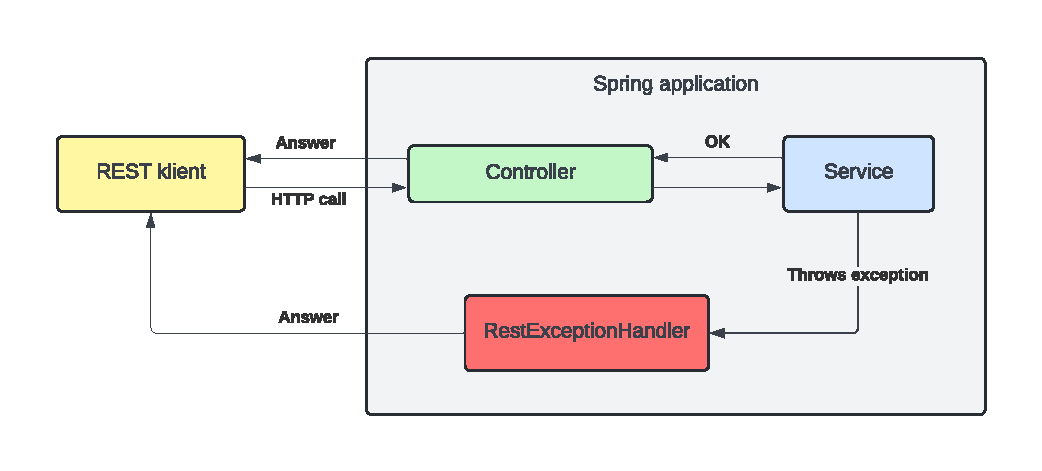
\includegraphics[width=0.9\textwidth]{figures/impl/API Implementation - endpoint.pdf}
    \caption{Obecný diagram koncového bodu}
    \label{fig:endpoint:general}
\end{figure}

Anotací \texttt{@RestController} určíme, že tato třída bude obsahovat koncové body. Dále pomocí anotace \texttt{@RequestMapping} zadáme cestu, pod kterou budou všechny koncové body v této třídě dostupné. A na závěr pomocí jednotlivých mapping anotací (\texttt{@GetMapping, @PutMapping @PostMapping @DeleteMapping}) určujeme, na jakou HTTP metodu má funkce reagovat.

Při mapování můžeme používat jak URI vzory pomocí regex výrazů (např \texttt{"/resources/*.png"}) tak i proměnné v URI (např \texttt{"/resources/{id}"}). Ten používáme třeba zde na výše zmíněném výpisu kontroléru postavy \coderef{code:characterController}[, řádek 9] pro získání jedné entity \textit{Character}. S tím se pojí anotace \texttt{@PathVariable}, která určuje, že vstupní parametr id bude brán z URI a bude se jednat o datový typ \texttt{int}.

Jako další můžeme používat tzv. \textit{query} parametry, které je možné získat získat za pomocí anotace \texttt{@RequestParam}, kde se může předem určit, zda je parametr povinný nebo jakou bude mít výchozí hodnotu \coderef{code:characterController}[, řádek 12]. Ve výsledné URI požadavek pro získání entity s identifikátorem 1 a načteným inventářem bude vypadat následovně: \texttt{GET /characters/1?include=inventory\&} \texttt{lazy=true}. Tento požadavek vrátí postavu hráče s namapovaným inventářem a s ostatními atributy. Atributy \textit{clazz} a \textit{race} \figureref{fig:dix:database_schema}
budou vypsané pouze jako id a nebudou nainicializované.

Pro metody post byla ještě použita anotace \texttt{@RequestBody}, pomocí které můžeme vzít data z těla požadavku. V našem případě jsme požadovali JSON objekt, který se hned mapoval na objekt třídy.

\begin{listing}[h!]
    \inputminted[]{Java}{resources/code/impl/CharacterController.java}
    \caption{Kontrolér pro entitu \textit{Character}}
    \label{code:characterController}
\end{listing}

\subsubsection*{Popis výsledných koncových bodů}\label{sec:impl:endpoints:desc}   %%TODO barče prosím prosím odsud po další kapitolu
Koncové body u metody GET obstarávající základní zobrazení entit v databázi (např. \texttt{/actions/1}) mají implementován lazy load \subsectionref{sec:impl:lazyload} s možností vypsat pouze námi určené atributy. Pokud si tuto možnost uživatel zvolí, ostatní atributy, které jsou objekty, zde budou mít pouze ID \coderef{code:action:endpoint:single}. Když žádné parametry nespecifikujeme, předpokládá se, že chceme celý objekt se všemi načtenými atributy.

\begin{listing}[H]
    \begin{minted}{json}
// /actions/1?lazy=true&include=attack 
{ // for simplicity there are only important fields
  "id": 10,
  "title": "Fireball",
  "skill": 2,
  "attack": {
    "id": 6,
    "range": 4,
  }
}
    \end{minted}
    \caption{Příklad URI a odpovědi pro získání entity s identifikátorem 1 a načteným atributem \textit{attack}}
    \label{code:action:endpoint:single}
\end{listing}

Koncové body pro metodu GET, které vrací více objektů, jako například \texttt{/actions}, mají kromě výše zmíněné možnosti výběru atributů také možnost stránkování. Za pomocí něj můžeme například vzít pouze prvních pět objektů a tím zmenšíme potřebné zdroje pro přenos. Tato funkcionalita vrací kromě objektů taktéž informace o tom, na jaké stránce se nacházíme \coderef{code:action:endpoint:multiple}. Samotné objekty jsou uloženy v poli \texttt{entries} a mají stejný formát, jako výše zmíněný výstup pro jeden objekt \coderef{code:action:endpoint:single}.

\begin{listing}[H]
    \begin{minted}{json}
// /actions?page=2&limit=5&include=attack&lazy=true
{
  "pagination": {
    "count": 5,
    "hasMoreEntries": true,
    "totalEntries": 54,
    "page": 2,
    "limit": 5
  },
  "entries": [ 
    // 5 single objects
  ]
}
    \end{minted}
    \caption{Příklad URI pro získání pěti objektů od 6 do 10 a načteným atributem \textit{attack}}
    \label{code:action:endpoint:multiple}
\end{listing}

Vytvářecí metoda POST poté bere jako vstupní parametr v těle požadavku objekty, které se mají vytvořit, a dotazuje se na množné číslo URI (např. \texttt{/actions/}). Metoda PUT pro úpravu dat bere taktéž objekt, který se má upravit, v těle a navíc v URI se specifikuje ID objektu (např. \texttt{/actions/1}). A nakonec metoda DELETE bere jako URI parametr pouze ID objektu, který se má smazat (např. \texttt{/actions/1}).

Celkový seznam všech koncových bodů s popisem je zapsán v Tabulce \ref{tab:endpoints}. Poté ještě byla vytvořena dokumentace pro koncové body pomocí frameworku Swagger \sectionref{sec:impl:swagger}, které je možné nalézt na adrese \url{https://api.tts-game.fun/swagger-ui/index.html#/}.


\section{Testování}\label{sec:testing}
Testování probíhalo za pomocí dobrovolníků, kteří si zkusili zahrát hru, nebo díky dokumentačnímu rozhraní Swagger \sectionref{sec:impl:swagger} pohodlně testovali přímo koncové body v API.



\section{Problémy při vývoji}\label{sec:impl:problems}
Během vývoje se vyskytlo několik problémů, které se musely vyřešit. Nyní se zaměříme na ty nejzávažnější.

\subsection{Serializace}
Když byly atributy označeny jako \texttt{lazy}, pořád byl problém při serializaci, kdy k těmto atributům knihovna Jackson přistupovala, čímž byly načteny z databáze a následně serializovány, i když se v kódu s nimi nepracovalo. Tento problém byl vyřešen pomocí vlastní třídy \texttt{LazyFieldsSerializer}
na serializování namapovaných objektů. \sectionref{sec:impl:serialization}

\subsection{Lazy load}
Knihovna Hibernate bohužel nemá metodu pro rekurzivní načtení relací objektu, v souvislosti s vlastní serializací pak nastal problém, když se měl serializovat objekt se všemi jeho relacemi. Hibernate podporuje jen načtení objektu který je instancí \texttt{HibernateProxy}. Tento problém byl vyřešen pomocí statické funkce \texttt{hibernateInitializeAll()}. \sectionref{sec:impl:lazyload}

\subsection{Příliš velká databáze}
Při návrhu databáze nebyl brán ohled na možnou časovou náročnost. Databáze se navrhovala jako funkční celek připravený do produkce s ohledem na případné rozšíření. To vyústilo v problém, kdy jednotlivé případné úkony jako je \gls{orm} či \gls{crud} operace nad jednotlivými entitami byly velice zdlouhavé a zabíraly většinu času vývoje. S tímto se pojil o to složitější management změn u koncových bodů. Z tohoto důvodu se v implementaci vynechaly entity \textit{summon} a \textit{item}.

\subsection{Začátek návrhu od databáze}
Před začátkem práce nám bylo doporučeno, abychom jako první provedli návrh databáze. Toto rozhodnutí se ovšem v pozdní fázi vývoje ukázalo jako velice nepraktické, protože při mapování se musely M:N relační tabulky obstarat ručně. Kdybychom začali s vývojem databáze přímo v aplikaci, knihovna JPA \sectionref{fig:JPA} by za nás obstarala M:N relace, čímž by se implementace upravování a vkládání nových vnořených objektů podstatně zjednodušila. Vzhledem k počtu m:n relací, které databáze modelové hry obsahuje, by se tímto jednalo o velkou úsporu času.
\chapter{Závěr}
Tato práce se zaměřila na návrh a implementaci aplikačního rozhraní pro hybridní deskovou výpravou hru. Cílem práce bylo vytvoření \gls{api} pro hybridní výpravnou hru, která kombinuje jak fyzické tak virtuální prostředí, s podporou pro administrátorské rozhraní a uživatelské prostředí. Během práce byla provedena analýza již existujících řešení a standardů, které byly následnou inspirací pro návrh a implementaci vlastního řešení.

Implementace zahrnovala vytvoření \gls{restful api}, které je založeno na frameworku Spring Boot a využívá databázi pro ukládání dat. \gls{api} bylo navrženo s ohledem na bezpečnost, unifikaci a jednoduchost použití. Pro dokumentační rozhraní byl využit nástroj Swagger. 

Součást této práce byla také spolupráce mezi jednotlivými členy týmu, zvláště při prvotním návrhu databáze a funkcionalit modelové hry. 

Jako vedlejší produkt této práce je i příručka \gls{api} vygenerovaná za pomocí nástroje Swagger, která je dostupná na jednom z koncových bodů \gls{api}.

Celkově lze tedy konstatovat, že cíle této práce byly splněny a výsledkem je funkční \gls{api} pro hybridní výpravnou hru. Vzhledem k tomu, že se při návrhu bral ohled na případnou rozšiřitelnost, je možné hru obohatit o další funkcionality. Rozvinutí této práce by se mohlo zaměřit na rozšíření či optimalizaci zpracování současného \gls{api}.

\endinput



% Seznam literatury
\printbibliography[title={Literatura}, heading=bibintoc]


% Seznam zkratek
\printnoidxglossary[type=shortcuts]%, style=shortcuts]
\printnoidxglossary[type=term]%, style=shortcuts]

% Přílohy
\appendix
\input{chapters/appendix/implProblems}
\begin{figure}[h]
    \centering
    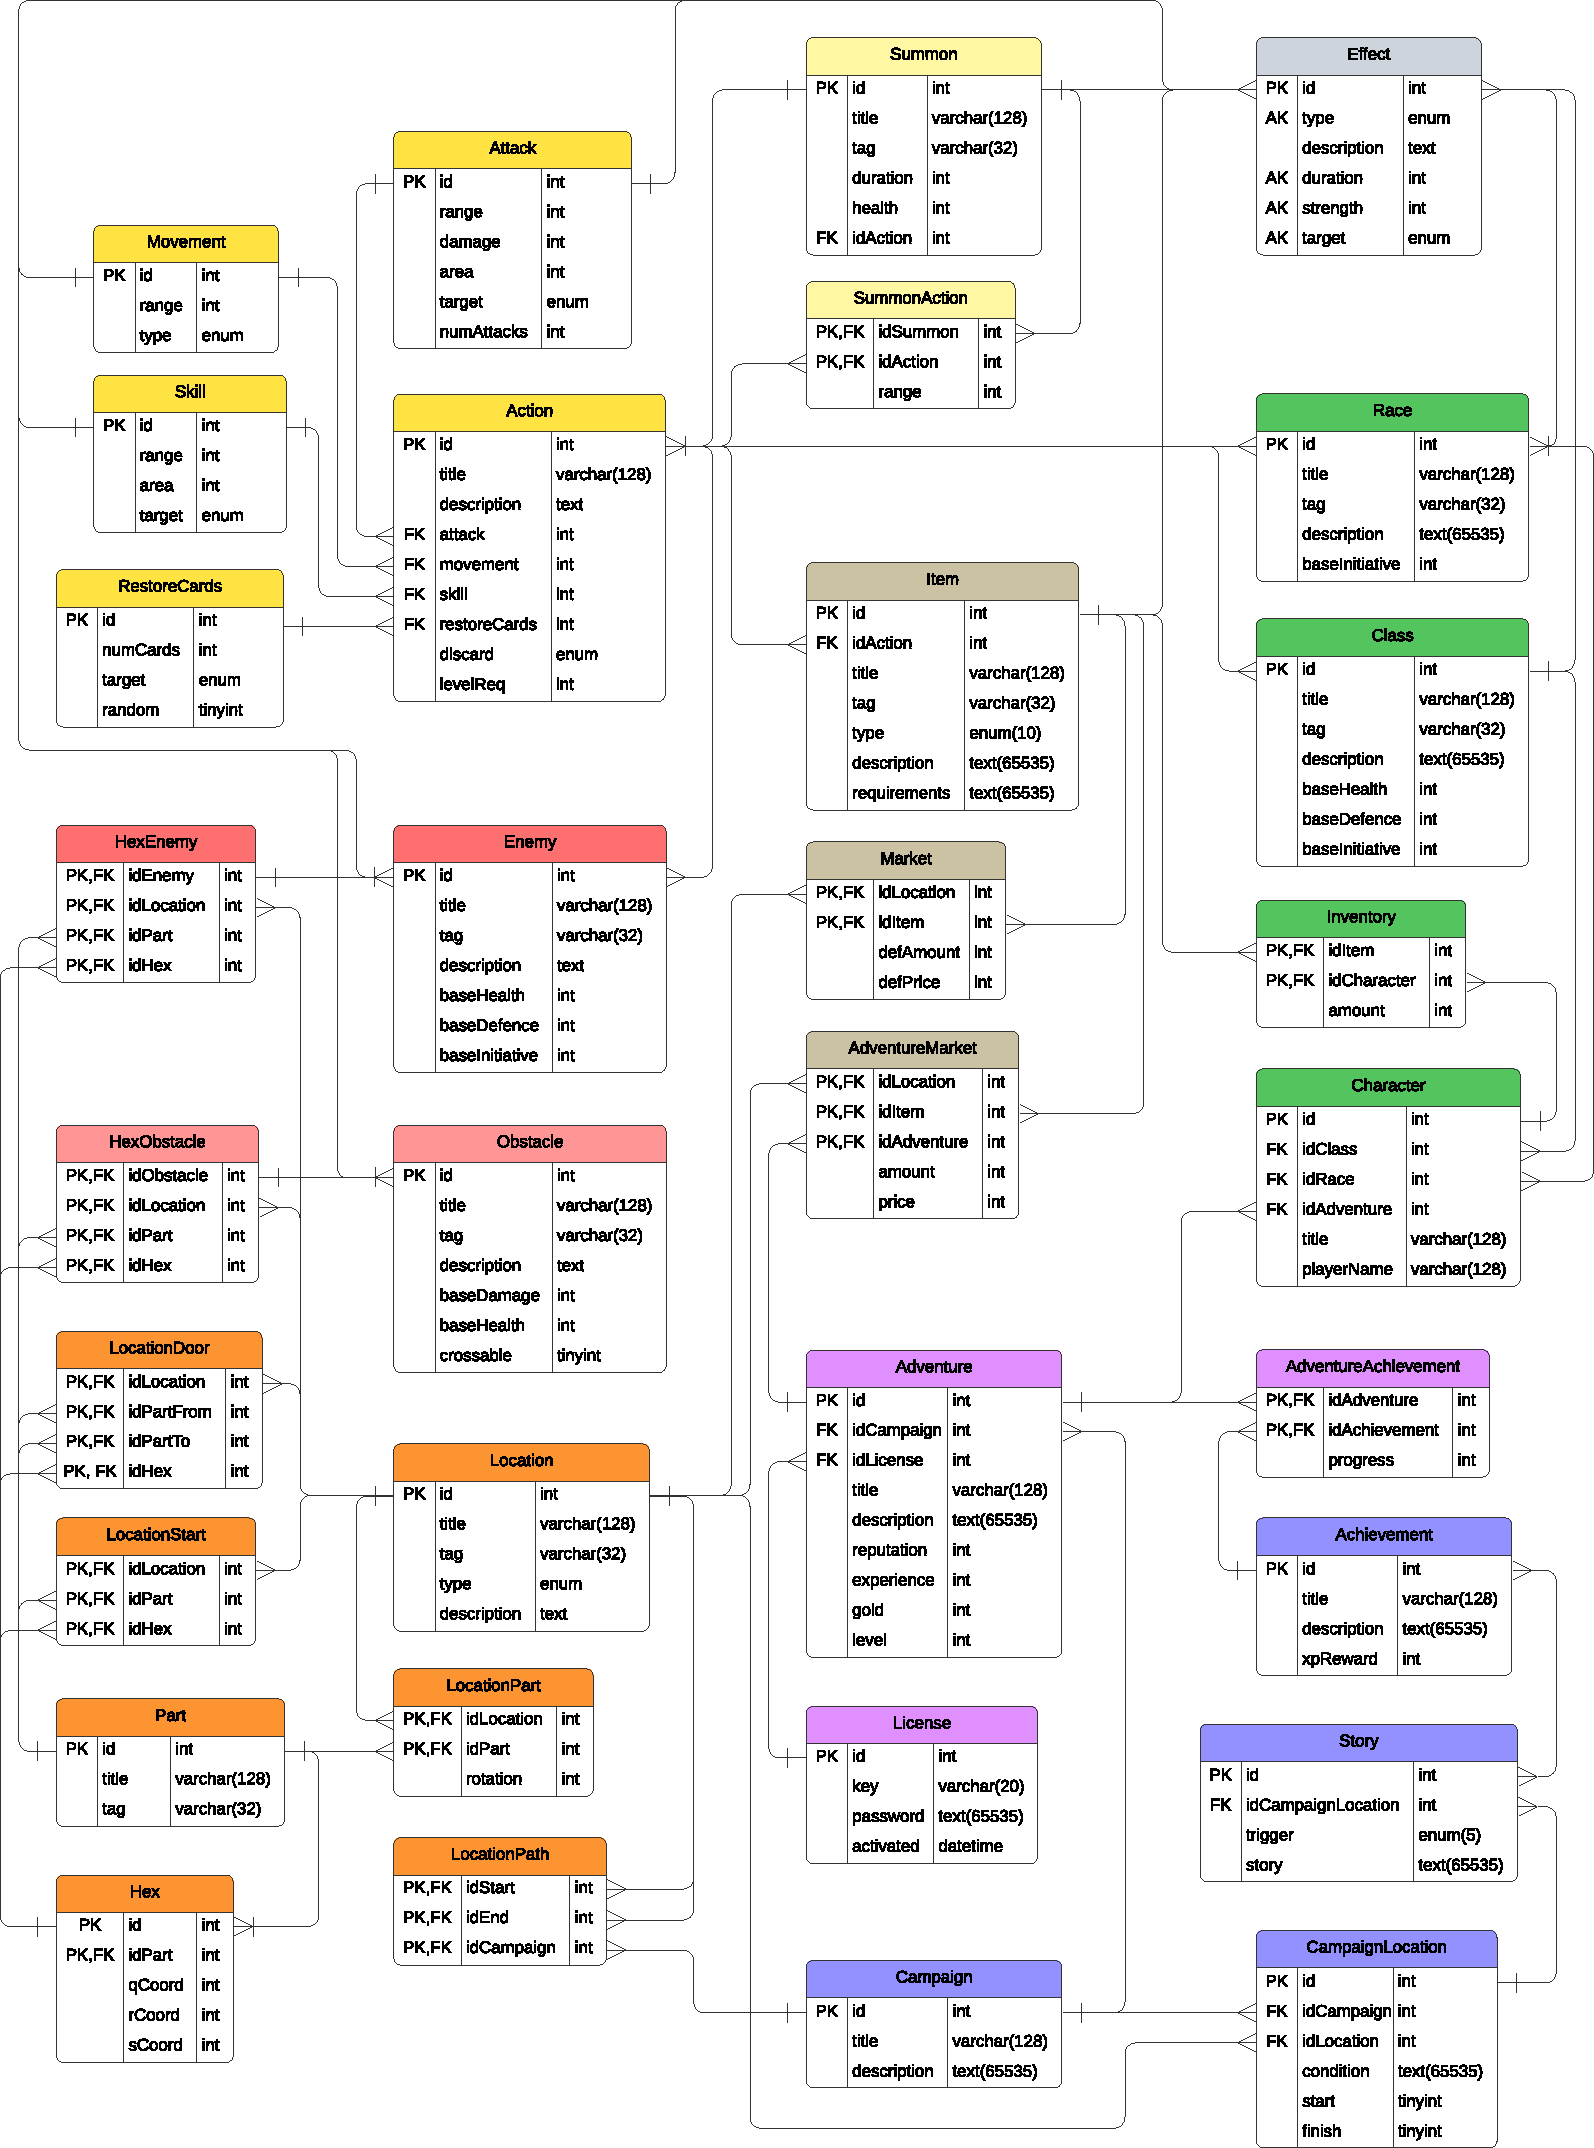
\includegraphics[width=0.9\textwidth]{../../shared/diagrams/dbScheme.pdf}
    \caption{ER diagram databáze}
    \label{fig:dix:database_schema}
\end{figure}

\end{document}
